% Thesis framework file. See individual files for details.
\documentclass{iitkgpthesis}

\usepackage{pifont}
\usepackage{amsmath}
%\usepackage{amssymb} %for >=
\usepackage{mathtools} %for dcases and condition
\usepackage{amsfonts} %for \mathbb{}

%\usepackage{natbib}
%\usepackage[sort&compress,square,comma,authoryear]{natbib}

%\usepackage[square,sort,comma,numbers]{natbib} %for bibliography
% package used by \citep and \citet
%\usepackage[sort&compress,square,comma,authoryear]{natbib}

% makes color citations
%\usepackage[dvips,dvipdfm,colorlinks=true,urlcolor=blue,citecolor=red,linkcolor=red,bookmarks=true]{hyperref}




\begin{document}
\cleardoublepage
% Frontmatter. Add other pages as needed.
\pagenumbering{roman}

 % Page 1 : Main Text
\thispagestyle{empty}
\begin{center}
% \textbf{\large Area Sweep Coverage in Wireless Sensor Networks }
\textbf{ \LARGE{SPATIAL DATA: CRAWLING, METADATA DISCOVERY, PUBLISHING \& QUERY ORCHESTRATION} }
\end{center}
 \vspace{-2.5em}
\begin{center}
% \textbf{Geo-Service Portal -- Foundation Platform}
\end{center}
 \vspace{-2.5em}
\begin{center}
\textbf{\large Geo - Service Portal }\\
% \textbf{ Foundation Platform }
\end{center}
% Uncomment the following if a third line is required
%  \vspace{-2.5em}
% \begin{center}
%  \textbf{\large FOLLOWED BY THE THIRD ONE}
% \end{center}
 \vspace{2em}
\begin{center}
 \textbf{\textit{Thesis submitted to Indian Institute of Technology Kharagpur}} 
\end{center}
 \vspace{-3em}
\begin{center}
 \textbf{\textit{in partial fulfillment of the requirements for the award of the }} 
\end{center}
 \vspace{-3em}
\begin{center}
 \textbf{\textit{degree of}}
\end{center}
 \vspace{-1em}
\begin{center}
 \textbf{ Master of Technology}
\end{center}
\vspace{-3em}
\begin{center}
 \textbf{\textit{in}}
\end{center}
 \vspace{-3em}
\begin{center}
 \textbf{{Information Technology}}
\end{center}
 \vspace{-3em}
\begin{center}
 \textit{by}
\end{center}
 \vspace{-1em}
\begin{center}
 \large{\textbf{Punjabi Deepak Bharatbhai}}
\end{center}
 \vspace{-3em}
\begin{center}
 \large{\textbf{15IT60R17}}
\end{center}
 \vspace{-1em}
\begin{center}
 Under the guidance of
\end{center}
 \vspace{-2.5em}
\begin{center}
 \large \textbf{Prof. Soumya K. Ghosh}
\end{center}
 \vspace{0em}
\begin{center}

\includegraphics[scale=0.15]{images/logo.png}
\end{center}
 \vspace{-1em}
\begin{center}
 \textbf{\small DEPARTMENT OF COMPUTER SCIENCE AND ENGINEERING}
\end{center}
 \vspace{-3em}
\begin{center}
 \textbf{\small INDIAN INSTITUTE OF TECHNOLOGY KHARAGPUR} 
\end{center}
 \vspace{-3em}
\begin{center}
 \textbf{\small APRIL 2017}
\end{center}
 \vspace{-1em}
\begin{center}
 \copyright 2017 Deepak Punjabi. All rights reserved.
\end{center}

\clearpage
%\newpage
%\thispagestyle{empty}
%\cleardoublepage

 % Page 5 : Certificate on department letterhead
\thispagestyle{empty}
{~} % Buffer blank character to prevent horizontal underflow due to next \vspace
\vspace{10em} % Increase if the dept. letterhead requires more space
\begin{center}
\textbf{\large CERTIFICATE}
\end{center}
This is to certify that the thesis titled \textbf{Geo-Service Portal}, submitted by \textbf{Deepak Punjabi}, in the Department of Computer Science and Engineering, Indian Institute of Technology, Kharagpur, for the award of the degree of Master of Technology, is a record of research work carried out by him under my supervision and guidance.

The thesis fulfills all the requirements as per the regulations of this institute. Neither this thesis nor any part of it has been submitted for any degree or academic award elsewhere.
\\
\\
\begin{flushright}
\textbf{Prof. Soumya K. Ghosh}\\
\textbf{Dept of Computer Science \& Engineering}
\end{flushright}

\clearpage
 % Clear any double page gaps
%\newpage
%\thispagestyle{empty}
%\cleardoublepage




 % Page 11 : Abstract
\thispagestyle{empty}
\begin{center}
\textbf{\Large Abstract}
\end{center}
In the recent era of technology data is everything. One of the very useful type of data is spatial data. The information about spatial data can be found to be much useful in many fields of industry. From remote sensing, mining to doing spatio-temporal analysis to doing flood or disease spread analysis, the applications are endless. However this data is not generally publicly easy to find. Spatial data is not handled well by the the general purpose search engines. The methods to access these data are also heterogeneous and many times require licensing and using proprietary technologies. Heterogeneity of the data poses another problem of ranking and combining  A central catalog service can be built to keep track of this various repositories, also the data can be made available through simple unified calling mechanisms. With the availability of large amount of heterogeneous data from different multiple sources one can do many type of spatio temporal analysis. This catalog service can then behave as central node for all available geo-spatial data available in the web. Registry can be used to publish all the information to subscribers and open web. Using this registry an efficient query processing system can be built around it to generate information needed in the user friendly mode. Query processor can find data from various heterogeneous data stores and process the data to get one result from many data sources. Various ranking and cost matrices can be deployed to make indexing of returned data feasible.
\newpage
\thispagestyle{empty}
%\clearpage
%\cleardoublepage

 \tableofcontents
 \listoffigures
\newpage
 \thispagestyle{empty}

%  \include{listofnotation}
%  \listoftables


% Main thesis section
\pagenumbering{arabic}
\pagestyle{plain}
\chapter{Introduction}

As the information around us grow exponentially, spatial context about such information is becoming more and more important and useful. For example, If one wants to go from one place to other, He or she always chooses the path that is spatially shortest. Another good spatially aware example is when a person wants to buy a house. Many factors affecting the decision to buy a house are inherently spatially aware, like how far is the hospital, how far is the school facility or is there any good restaurants available nearby. All these examples suggests that one of the crucial factor while buying a house is how qualitative is the spatial neighbourhood. Or we can say that many decisions occurring in everyday life of a person are spatially aware.
\newline
\par
It can be said that spatial data is another dimension for organizing information. With this, getting and organizing spatial data for yielding useful information becomes more and more useful. This creates a desired motivation for building such system to effectively collect and utilize spatial data.


\section{Motivation}
Currently available search engines are good for normal data such as text and web links, but when it comes to searching and ranking spatial data, none of the currently available search engines can provide efficient results. One of the reason for this can be that not all Geo-spatial data is publicly available. Other problems is that repositories containing spatial data are not generally indexed and the meta-data information about what data they contain is not easily available. Also the normally crawled data is not kept in a spatially aware manner. Our motivation here is to build a registry service that can crawl spatial data from the open web, avail data from national government agencies as well as open source free repositories. Once the data is available various kinds of tasks can be built on top of that. This behaves as a foundation platform to provide basic and robust services upon which various other services can be built. We call this as Geo-Service Portal. One can easily build and perform various type of spatial queries like GetMap on the data available. Various graphical applications as well as application programming interfaces(APIs) can be provided on the available data to cater in use in various ways. A query interface can be built upon the data available from catalog service. This query interfaces can provide various views for user specific user queries. An spatial-temporal analytics can also be done using the catalog. Change of data can be tracked. Other use cases can be finding the spread of diseases or getting the area affected by flood. Many other applications can be generated.

\section{Problem Statement}
The aim of this project is to create a foundation platform for crawling, storing, maintaining and publishing meta-data information about spatial data and corresponding providers and to utilize this information to perform efficient query orchestration.


\section{Objectives}

\begin{enumerate}

\item \textbf{Build a topical crawler to crawl the web and store Geo-spatial metadata.}
\par
\indent A topical crawler is a special type of crawler which only searches for information of a particular topic interest. Here the topical crawler crawls the open web, finds and filters URLs found by it. This module checks whether the server provided by the URL is capable of providing OGC compliant geo-spatial web services or not. If the URL is found to be a geo-server it stores all the metadata information about the Geo-server and about the data it contains into the database. It uses domain ontology knowledge to classify data into different domains. This information then later can be utilized to query and find useful information.
\newline
\item \textbf{Build an OGC compliant catalog service to publish and search accumulated metadata.}
\par
The aim here is to build a web service that can query and publish relevant metadata information from the database. The catalog service is real-time. The data stored in the catalog changes with time to reflect changes in corresponding data from the providers. This can also be explored to examine spatio-temporal nature of the data. The catalog service should be built in such a way that queries can be processed in real time. For this purpose the data should be stored in database in structured manner rather than storing it in plain json or XML files. The responses provided by the spatial repositories are generally in XML, GML or shape format, catalog service parses the data to store data in a structured way in database so that various query operations can be supported in OGC compliant manner. One other crucial point for catalog service is to provide high availability. Registry is used to search as well as publish the available data.\\
\begin{figure}[h]
  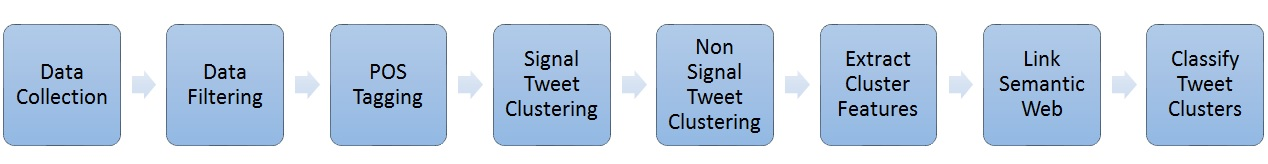
\includegraphics[width=\textwidth]{pix/flow}
  \caption{3 - staged pipeline approach}
\end{figure}
\newline
\item \textbf{Build Query orchestration service to perform real-time query with heterogeneous data sources and cost matrices associated with them.}
\par
One of the tasks of catalog service is to provide relevant information to the querying machine or person. The data that is stored by different repositories can be of heterogeneous form. Task of query orchestration is to find relevant information across all available data sources and perform the query using all relevant data. If the data is available from multiple data sources different type of ranking and cost matrices can be associated to provide most relevant information to the user. Query orchestration is also associated with ranking. While retrieving the data it should be presented to user in a ranked retrieval manner based on some metrics. Here we have discussed two techniques of ranked retrieval and indexing called Quad tree based indexing and ranking based on quality preferences.
\end{enumerate}

\section{Organization of thesis}
This thesis is mainly organized into six chapters. The first chapter gives introduction about the subject matter, it clears the motivation and advantages of the project. It defines the problem statement and states as well as explains the objectives of the project. The second chapter namely literature survey, provides already available data about the subject and proposed solution methods. This section first explains about the data for the model to be work with. It explains the web services and APIs build for spatial data. Then it explains about three part of the foundation platform, Spatial web crawler, Catalog service and query orchestration. Chapter 2 also discusses about the previous work done in the respective fields. 
\newline
\par 
Chapter 3, 4 and 5 are the core foundation blocks for Geo-service portal foundation platform. Chapter 3 is explains about the spatial web crawler. It explains the architecture and the algorithm used for the spatial web crawler. It also explains advantages of spatial web crawler. Chapter 4 contains information about spatial metadata discovery and publishing. It discusses objectives for the catalog service. It also give architecture and implementation details about catalog service for web and query processing. It also shows example results. It also extends the concept to cloud based paradigms.Chapter 5 gives a look into spatial query orchestration. It discusses about two broad strategies two index and rank spatial data.
\newline
\par
The final chapter concludes the morals of the thesis and creates a pathway for better optimizing and extending the proposed solution for the future work.
% \section{Development Platform}
\chapter{Literature Survey}
The literature for this project can be divided mainly into four parts. The spatial data and spatial web services on which the framework is developed. Crawling: How to find that data. Catalog Service: Once the data is found, how to store that data. How to make data easily accessible to others. And at the last Query orchestration: how to perform simple queries on the available data.

\section{Spatial Data \& Spatial Web Services}
\par
The term Geo comes from geography. Geography stores all the information of location and shape of the object in the spatial data. Spatial data stores the relationships between these data. It can also be easily mapped to a map. Spatial data is stored as raster data or vector data. Geo-server provides various kinds of functionality to this type of data. Spatial data is the data that can be mapped.Spatial data is collection of spatial object that has topology and co-ordinates. Spatial data gives geographical and shape related attributes of the data.Geographical information system is used to retrieve and operate on spatial data. Different operations can be add, visualize, annotate etc. A Geographical Information System provides various extended operation on spatial data. Different examples of such software that offers spatial services are ESRI, Microsoft SQL Server, ERDAS imagine etc.

\subsection{Classification of Spatial Data}
Open Geo-spatial Consortium(OGC) defines  Different types of object under the class geometry are as below. All the major Geo-spatial service providers and vendors provide this kind classification.The primitive four data types in spatial data are point, curve, surface and GeomCollection. Figure \ref{cosd} shows hierarchy in classification of spatial data.\\
\newline
\begin{figure}[h]
    \centering
    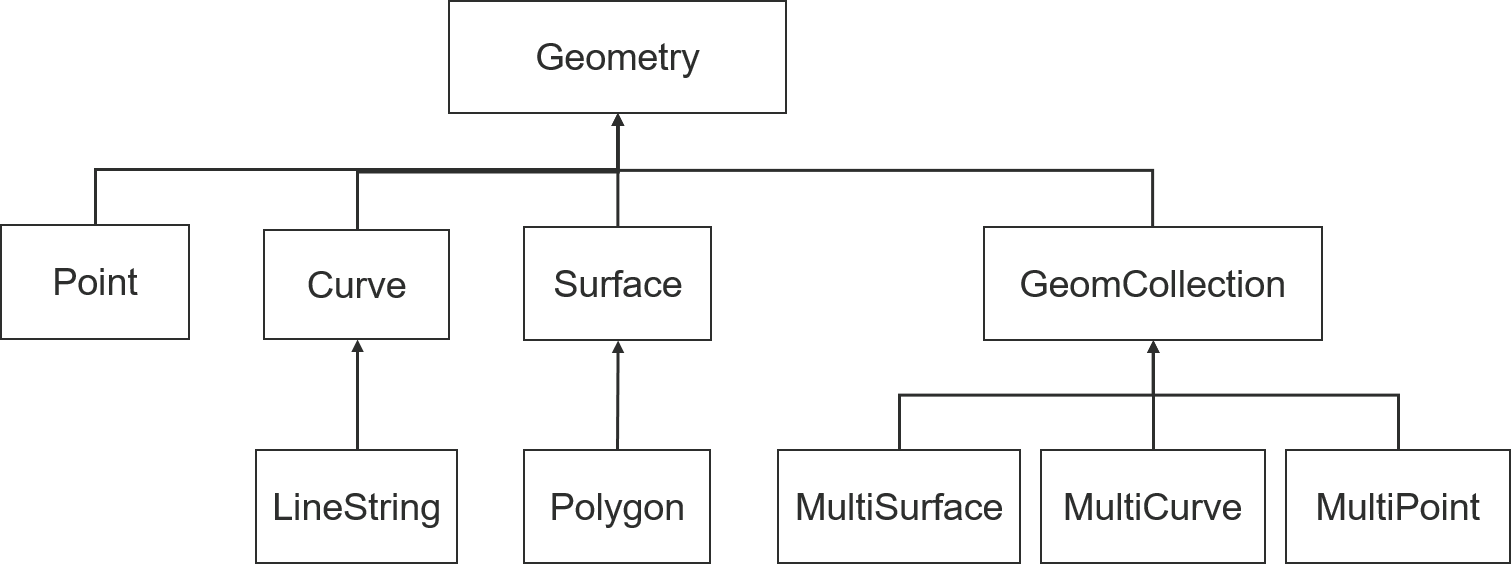
\includegraphics[width=\textwidth]{pix/p}
    \caption{Classification of spatial data}
    \label{cosd}
\end{figure}
\newline
\begin{itemize}
\item \textbf{Point}\\
Point in a map is denoted by (x, y) co-ordinates. When we see kharagpur city on a scale
of India it will be seen as a point. Point can be used to denote various objects like origin,
city, end point, top of the mountain etc. It denotes a single point consisting of longitude and latitude.\\

\item \textbf{Curve}\\
Curve is used to denote collection of points. This can be a straight line or curve. For
example, a road network can be represented with the help of line strings. Similarly, a
river can be denoted as a curve. Curve can be made with help of two distinct points.\\

\item \textbf{Surface}\\
A surface is representation of an area or a polygon. When kharagpur is seen in the scale
of west Bengal it is seen as surface or polygon. Polygon can be made using at least three non-linear points. Every polygon has a feature called boundary.\\

\item \textbf{GeomCollection}\\
Collection of basic building blocks defining a new type of geometry can be defined
with the help of GeomCollection. GeomCollection is made with combining two or more geometry types.\\

\end{itemize}


\subsection{OGC Web Services}
Open Geospatial Consortium (OGC) is the worldwide standardization body for geospatial standards. OGC provides a standardized way of accessing this geospatial data. OGC mainly provides three kinds of web services.\\
\begin{itemize}
\item \textbf{Web Map Service (WMS)}\\
Web Map service defines a way of accessing geospatial information across all geo servers in a
standard format as image. This image can be raster image or a vector image. Raster images are
of type jpg, png or bmp. Vector images contains svg format extension images. It also provides
a way to access metadata about the available information of the layers. This information can
contain type and no of layers. \\
Some of the well-defined operations in this layer are
GetCapabilities, GetMap and DescribeLayer. GetCapabilities operation returns capabilities of the server for example, what kind of services the server offers. This operation may be useful to check if a server is geo server or not by examining the kind of services it offers. GetMap service returns map images for the queried data. multiple such layer of images can be queried and then can be overlaid on top of each other. for example satellite view, terrain view, traffic view etc. Each of this layer gives additional information to the map. DescribeLayer operation describes what are the available layers and what is the metadata about the layers.\\
\item \textbf{Web Feature Service (WFS)}\\
WFS allows direct access to features contained in the map. WFS uses SOAP based interface. SOAP is used to minimize the overhead into the communication and verify cross platform stability.
For exchanging data between client and server WFS uses Geographical mark-up language(GML)
which is based on XML. Some well-defined operations in WFS are query or get feature, which
returns the feature stored on the server. We can add the feature in the repository by add feature.
We can delete feature by delete feature. Also we can update feature stored in the repository by
update feature. We can also lock certain feature to disallow modification of it while sharing via lock feature. Locked resources and features wont be accessible to change to other clients. Example of feature are the objects in the map like building or petrol pump.\\
\item \textbf{Web Coverage Service (WCS)}\\
WCS offers multi-dimensional coverage of the geo spatial data.It can provide originally retrieved data or provide processed data. It provides spatio-temporal
context to the given geographical data. For example, it can show the flow of the river changing
over the span of years. Thus we can say that WCS provides richer coverage of spatial data than
WFS or WMS. Coverage data is mainly used for scientific calculations.
\end{itemize}
\section{Spatial Web Crawler}
Spatial web crawler is a topical crawler which finds geospatial capable servers and services from the web. Sonal Patil\cite{l1} provides the base architectural guidelines for building spatial web crawler. Wenwen Li\cite{l2} says that if a server is offering geo-spatial capabilities then it can be either of the WMS, WFS or WCS server. The geo-servers must comply to OGC standards for geospatial data. This can be checked using GetCapabilities service request. We can check whether a given server offers WMS offerings or not can be checked using special suffix string added to the URL of a geo-server. More details are covered in the geo-spatial crawler part below. If the server is indeed a WMS server, It replies with and XML files containing all the data and operations it can offer. We call this as services.xml file. Once We know that the server is a geoserver many kinds of operations can be performed on it. WMS geoserver offer various operations such as GetMap, DescribeLayer, GetCapabilities etc. WMS capabilities file contains all these operations mentioned above. This is to check if a particular server is geoserver or not. If we want to crawl through the open web, then we must repeat this process. For this purpose standard operation of crawlers are performed. We maintain a buffer of frontiers which divides the boundaries of crawled web and open un-crawled web. Wenwen Li\cite{l2} also suggests to make a auto updating crawler to periodically check whether there is any addition or removal or geoserver from the existing available data. This geoserver(s) also add new data to them and remove obsolete data from the data store. Automatic updates allows this operations to be done periodically and maintain the overall consistency of the data.\\
\par
Marc Najork\cite{l3} suggests that the task of crawling the web for WMS servers can be done parallel. He suggests to use parallel FIFO queues to carry out the operation efficiently. To check whether the URL already exists or not in the crawled set, he suggests to use efficient data structures to check set membership such as HashSet. He also suggests to use priority in crawling based on various methods such as PageRank.\\
\par
Lopez-Pellicer\cite{l9} suggests that there might be already available geoservers and catalog services on the web. We must efficiently identify this catalog services to different type of OGC compliant services. So that different kind of queries can be forwarded to different geo servers or catalog services. Dirk Ahlers\cite{l4} suggests an architecture to crawl and parse available geoserver(s) and store the available data efficiently. They also suggests to index the data so there data can be retrieved efficiently. This methods is described as focused crawling.\\
\par
Li, W., et al.\cite{l5} suggest a method to semantically crawls the web. In his approach he maintains a hierarchy of geospatial objects to identify parent children relationship. For example, river is a type of water-body. This kind of type of relationships can be used to manage and index available data and geoservers efficiently. JIANG Jun\cite{l6} suggests similar methods for WFS servers.


\section{Catalog Service for Geo-Spatial Data}
Catalog service provides discovery and publishing of geospatial metadata information. Manoj Paul\cite{l14} provides a service oriented approach for discovery and retrieval of spatial data as web services. Nogueras et al.\cite{l15} discusses about design and storage mechanisms in a real world catalog service. 
\newline
\par In this section we will look at two types of available catalog services for geospatial data. Python catalog service for web(PyCSW)\cite{l7} offers a model architecture for implementing a OGC compliant web service catalog portal. In this model, series of module are used to invoke a hierarchy such that decomposition of the functions and use case is efficient and easy. In this architecture many of the modules can work in parallel. Important modules are crawler, WMS capabilities files, Database to store geospatial data and a server to provide interface to functions. All the functions are implemented and run via programs on a server. This wsgi server acts as a geospatial catalog which accumulates data from various other geospatial repositories and catalogs available on the open web. Using the PyCSW interface many types of applications can be invoked. PyCSW provides various APIs for OGC compliant operations. For example, using GetMap a user or application can get all the data from all the crawled repositories in a single place. We can know the information available for the layers and from where this information is available. The detailed implementation of this architecture is discussed in the later chapters.\\
\par
GeoServer\cite{l10} also offers such services but it also offers powerful management tools and admin console to function via graphical user interface. It provides services to work with various data formats such as shape files or GML format, it supports various database options for storage purpose and it is extensible to add more services. In our approach, we will mainly use GeoServer as our catalog service. However it should be noted that GeoServer is more resource intensive than PyCSW as it provides more services than the latter. It provides integration with various programming languages like Python, Java, Ruby and PHP.
\section{Query Orchestration}
Query Orchestration provides query operations on the spatial data from the database. Various operations are available as OGC standards to operate and query on the data. Query orchestration also deals with indexing and ranking. Here we have used Quad tree for indexing spatial data. Quad tree\cite{l13} is particularly standard data structure for indexing spatial data. Another interesting concept is ranking by quality preferences\cite{l11}. In this concept we take the cumulative property of spatial neighbourhood to calculate ranking for the spatial objects. Ranking data by quality preferences is a advanced method and requires extra information about quality of data.\\
\par
Once the catalog service is built it can directly act as a single point for querying multiple repositories. The catalog server in-fact acts as a mediator while getting the queried data from other repositories. Different type of example queries are listed below.

\begin{itemize}
\item \textbf{Service metadata information}\\
Describes what kind of OGC compliant web services are offered by the catalog server or geo-server.
\item \textbf{GetLayers}\\
An interface can be built to provide information about list of available layers.
\item \textbf{GetOperations}\\
List of available operations can be provided that gives the information about the list of operations that are offered by the geoserver or catalog service.
\item \textbf{GetBoundingBox}\\
We can get the information about the bounding box of the layers or map that covers the total area.
\item \textbf{GetMap}\\
The map of particular layer can be retrieved.
\item \textbf{DrawMap}\\
The map of particular layer/data can be retrieved and placed onto another map. This is useful to find area of interest in the particular map by superimposing the queried data to generic map.

\end{itemize}
\input{chap21}
\chapter{Spatial Web Crawler}
Our first step to building the platform Geo-Service portal is to gather the required spatial data. This can be done by finding the available data sources for geo-registries from the web via crawling or adding the sources manually. Spatial data is not indexed and available as compared to normal image or text data. The crawler module crawls the open web to find OGC compliant geoservers and stores their metadata information. It uses ontology or hierarchical mapping or spatial data to classify the crawled features. This features are permanently mapped into ontology to help in query processing.

% ---------------------------------------------------------------
\section{Objectives}
\begin{enumerate}
\item Build a spatial web crawler which crawlers through available geo-servers which offers WFS
based OGC compliant services.
\item Build a domain specific vocabulary(ontology) for this features which can be helpful to
compare found features with wanted features.
\item Perform semantic matching of found features from crawled web-pages with given
ontology for filtering the correct features and storing them in the permanent repository.
\item Perform an evaluation of the given spatial web crawler using metrics and test URL seed
sets.
\end{enumerate}

% ---------------------------------------------------------------

\section{Architecture of the Spatial Web Crawler}
Our crawler contains three modules for crawling spatial features through the world wide web.
Some of the definition needed for understanding the working of spatial web crawler are:\\

\begin{figure}[h]
  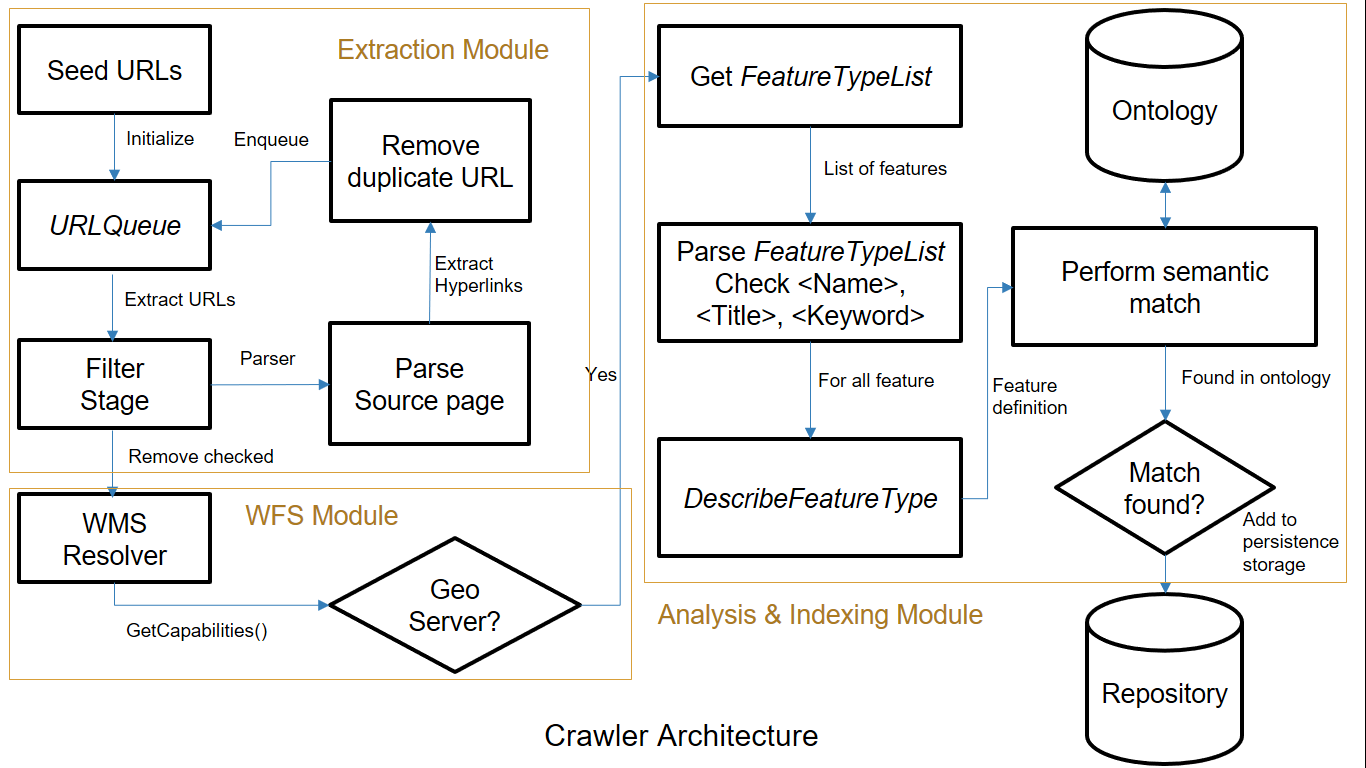
\includegraphics[width=\textwidth]{2}
  \caption{Spatial web crawler architecture}
\end{figure}


\begin{itemize}

\item  \textbf{Seed set}\\ A set of test URL(s) to initialize the queue for crawling the web. The crawler
starts with the URLs given in the seed URL set. Seed set URL(s) are processed and parsed to obtain other URL(s), which are added to the queue for later crawling.

\item \textbf{URLQueue}\\
A queue that contains set of URLs to be crawled. The crawler module takes URLs one after the another from this queue. It contains list of all the valid URL(s) to be crawled. It contains seed set initially. URL(s) are taken one by one by the crawler module for processing and deleted from the URLQueue. Similarly, newly found URL(s) are added to the queue.

\item \textbf{Frontiers}\\ 
A set of URLs from the URLQueue that are currently being crawled. This are
called frontiers because they reside between the known web and the unknown web. This are active URL(s) currently participating in the process of crawling. Frontiers are checked by the WMS resolver module for their geo-capabilities and parsed by extraction module to get new set of URL(s) to add in URLQueue.

\item \textbf{WMS resolver}\\
WMS resolver is a module that checks that if a server is WMS server
or not given the URL from the URLQueue. It uses special request URL to check whether the server replies to the URL in an OGC compliant manner. 

\item \textbf{Parser}\\
Parser is a module that downloads the webpage from the given URL and parse
the HTML webpage looking for pre-specified tags and names. After parsing it gets a
set of tags and its contents. In our implementation we parse the webpage and look for
the anchor tags within it and store all the hyperlinks from the crawled webpage. This links are then stored in the URLQueue for further processing.

\item \textbf{Ontology}\\ 
Ontology is a semantic dictionary containing all the features its type and relationship
hierarchy between features. This is used while mapping features to it's corresponding super-type and while query processing that contains more than one feature type. For example, getting overlap or intersection between two feature types.

\end{itemize}
Spatial Web Crawler is designed to contain three modules. This modules are namely Extraction module, WFS module and Analysis \& Extraction module. They are designed in a manner that they can work independently, which will come useful while implementing this as a extension in cloud based environments. :

\begin{itemize}

\item \textbf{Extraction module}\\
Our algorithm starts with a set of seed URLs contained in the seed set. We initialize the
URLQueue with these seed URLs. Initialization is done manually. It is required to choose these seed set URL(s) carefully, to get better results in crawling. Ideally, seed URLs should be good authorities, they should point to large number of good geoserver(s). Depending on the seed set, the crawler module may find more and less no of good spatial repositories in less or more amount of time. The crawler takes URL from the URLQueue and feeds it into filter stage. The filter stage takes the URL and checks
whether the given URL is already crawled or not. After filtering such URLs, they are sent to
the parser. The parser downloads the web-page from the given URL and parses it for finding
hyperlinks contained in it. These hyperlinks again go to filter stage for finding whether the
given URLs are already crawled or not. After filtering these URLs are added to the end of
URLQueue. The filtered URLs are also passed to the WFS module.\\

\item \textbf{WFS module}\\
Once the URL is fed into WFS module for the examination, WFS module sends a GetCapabilities() request to that server.
We do this by appending the request to the URL.
\begin{center}
$?
  service=wfs\&
  version=1.1.0\&
  request=GetCapabilities$
\end{center}
The server replies for this request. If the reply contains WFS\_Capabilities tag, then it offers
WFS service. We parse the received response for finding the WFS\_\\Capabilities tag. The server replies in XML format usually called capabilities.xml file, this files contains all metadata information about the feature services offered by the WFS server like number of layers, type of operations supported, feature description, etc. If the given
server is WFS server then the given URL is passed to analysis and indexing module.\\
\item \textbf{Analysis and Extraction module}\\
In this stage server response is parsed for the tag FeatureTypeList. FeatureTypeList
contains list of features. This features are stored under the tag FeatureType. FeatureType
tag contains set of keyword, title, name tags. Each of this tags are checked to see if it
contains any word from the ontology. For each of such tag found, DescribeFeatureType request
is appended to the URL.

\begin{center}
$“?service=WFS\&version=1.1.0\&request=DescribeFeatureType\&typename="+keyword$
\end{center}

Here the keyword is the name of the feature. Each of this retrieved feature is checked again
the ontology, if similar feature is found in the ontology then it is added to permanent storage in
the repository. Matching is done semantically via ontology. 
\end{itemize}

\section{Algorithm}
The \textit{Extraction algorithm} is used to crawl and parse webpages. It parses the available URL by downloading the webpage and extracts the anchor tags and corresponding URL(s) associated with it. It passes these URL(s) to \textit{WMS Resolver} module.
\newline
\begin{algorithm}[H]
	\caption{\em Extraction Algorithm }
	\textbf{Input:} set of URLs to start crawling \\
	\textbf{Output:} set of WMS capable URLs 
	%\begin{minipage}{\linewidth}
	\begin{algorithmic}[1]	 
	
	\algnewcommand{\Initialize}[1]{%
        \State \textbf{Initialize:}
        \Statex \hspace*{\algorithmicindent}\parbox[t]{.8\linewidth}{\raggedright #1}
        \newline
    } 
    
    \Initialize{
        \FOR{ URL in Input}
            \State $URLQueue.insert(URL)$
        \ENDFOR
    }
        
    \FOR{URL in URLQueue} 
        \IF{! filter(URL)}
            \STATE $preUrlSet \gets parser(URL)$
            \STATE $urlSet \gets filterDuplicate(preUrlSet)$
            \State $URLQueue.insert(urlSet)$
        \ENDIF
        \State $WMSresolver(URL)$
    \ENDFOR 
	\end{algorithmic}
\end{algorithm}
\par \textit{WMS Resolver} module checks if the URL provided by the \textit{Extraction algorithm} corresponds to a spatial repository or not. It does this via making standard OGC web service calls to the given URL. If The URL is found to be a spatial repository it is then forwarded to the Analysis and Indexing module. No actions are taken otherwise.
\newline
\begin{algorithm}[H]
    \caption{\em WMS Resolver Algorithm }
    \textbf{Input:} URL to check for OGC compliant services \\
	\textbf{Output:} WMS capabilities
	
	\begin{algorithmic}[1]
    \State $Response \gets GetCapabilities(URL)$
    \IF{$Response$ contains $WMS\_Capabilities$}
        \State $Analyze(URL)$
    \ENDIF
    \end{algorithmic}
    % \addtocounter{algorithm}{-1}
\end{algorithm}
\par The aim of \textit{Analysis \& Indexing} algorithm is to retrieve and store spatial features from the given URL. The algorithm first makes a request to get all \textit{FeatureTypes} from the spatial repository. For each \textit{FeatureType} it checks if the type matches semantically with the ontology. Matched features are stored into the repository.
\newline
\begin{algorithm}[H]
    \caption{\em Analysis \& Indexing Algorithm }
    \textbf{Input:} WFS capable URL \\
	\textbf{Output:} WFS records
	
	\begin{algorithmic}[1]
	    \State $FeatureTypeList \gets GetFeatureTypeList$
	    \FOR{ $feature in FeatureTypeList$}
	        \State $name \gets feature.name$
	        \State $description \gets DescribeFeatureTypeList(feature)$
	        
	        \IF{ $(name,description)$ matches in $ontology$}
	            \State Store record in repository
	        \ENDIF
	        
	    \ENDFOR
	\end{algorithmic}
\end{algorithm}

\section{Example Scenario \& Results}
Suppose we search for a example query after building the system. Let this query be \textit{river and snow}. Now if we search this on normal search engines like Google, it will show us results containing either river or snow. But as we have information about spatial context in this crawler. Repositories have stored the information about which features are in near proximity to each other.
\newline
\par
Other than this, we have a object ontology. Which is a hierarchical graph based on the spatial features. This graph contains generalized and specialized features. For example it suggests that river comes under the type stream which intern comes under the geometry type waterbody. This type of hierarchical classification helps us to understand the geospatial data and their features and relationships correctly. Our query is river and snow. The crawler searches the repository for finding both features river and snow or their similar representation by doing a semantic matching over ontology. Once found it can see which is the geo server which offers both of the geo services and feature types. Based on its finding from the repository we conclude our results and send the reply back to the user.
\newline
\begin{figure}[h]
    \centering
    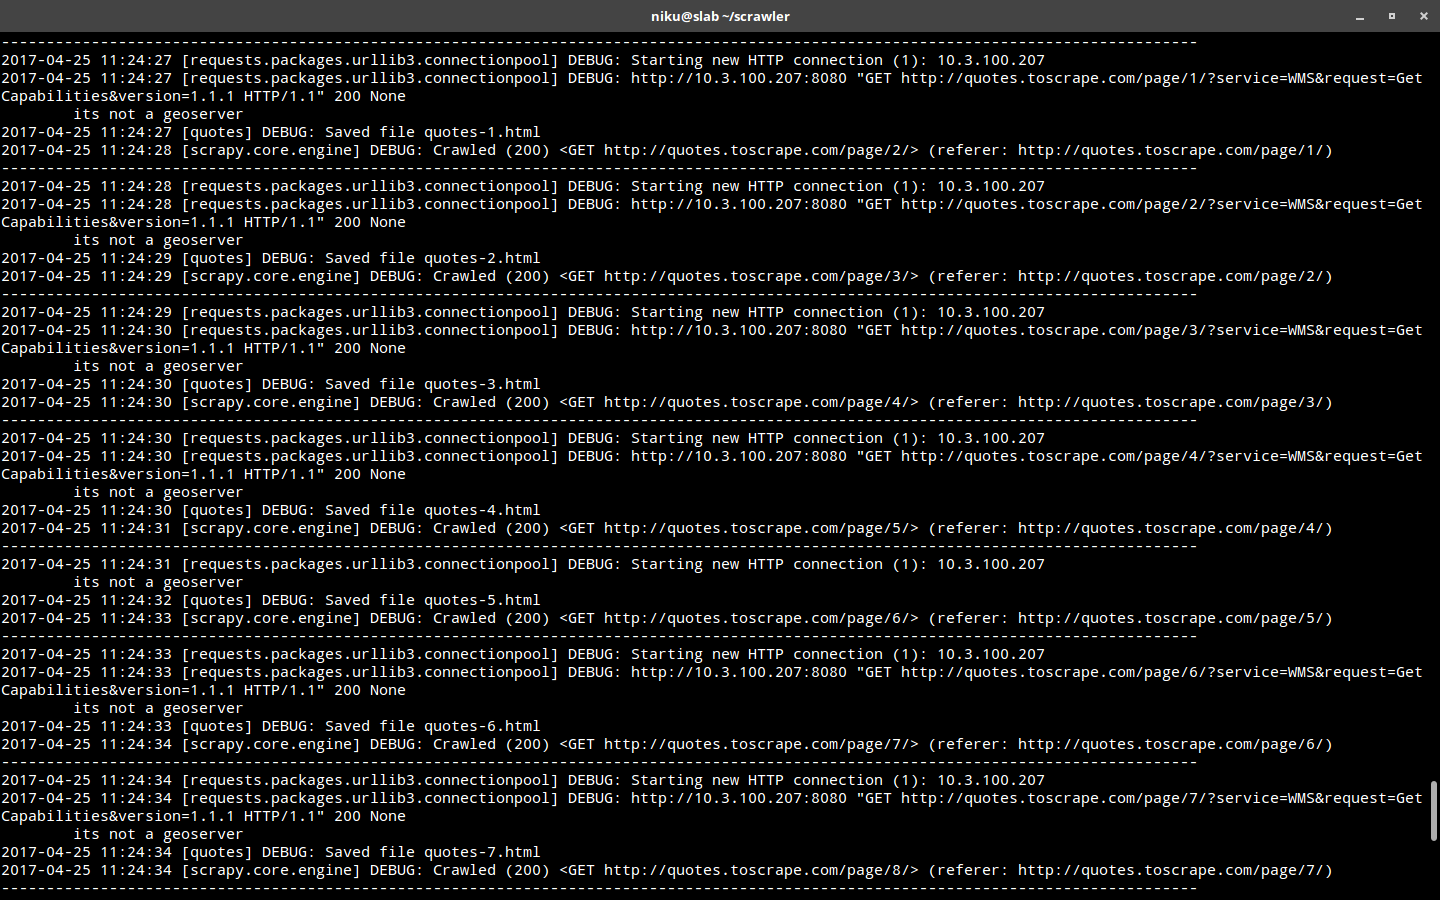
\includegraphics[width=\textwidth]{pix/p14}
    \caption{Spatial Web Crawler Implementation}
    \label{3.3}
\end{figure}
\newline
\par
Spatial web crawler is implemented with the help of Scrapy(\textit{https://scrapy.org/}) framework. It is a very powerful tool to crawl and scrap web pages. For each crawled URL, we pass it on the \textit{WMS\_Resolver} module to check if it is a spatial repository or not. Spatial GeoServer or catalog servers replies to GetCapabilities request with an XML file, part of which can be seen in the figure \ref{3.2}.
\newline
%%%%%%%%%%%%%% figure %%%%%%%%%%%%%%%%%%%%%
\begin{figure}[h]
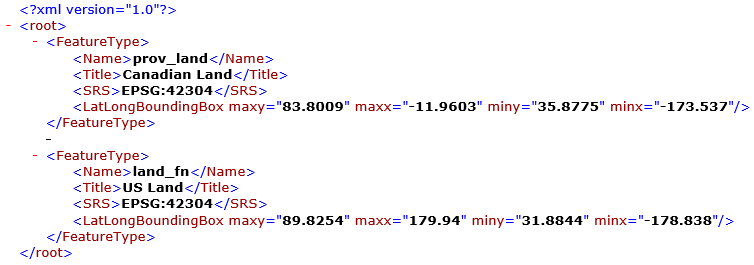
\includegraphics[width=\textwidth]{1}
\begin{center}
\caption{XML response from the geo server}
\label{3.2}
\end{center}  
\end{figure}
%%%%%%%%%%%%% figure end %%%%%%%%%%%%%%%%%%
\par
If the URL is not geo spatially capable, It is skipped as shown in the figure \ref{3.3}. For each URL the script prints if the URL is a GeoServer or not. If the URL is found to be a GeoServer, the response related to it is stored as XML and is further parsed and processed by catalog server.

\section{Advantages of Spatial Web Crawler}

\begin{itemize}
\item  Allows search in web pages that are not generally searchable from the normal search
engines. This is because of the spatial context awareness of the spatial web crawler.
\item It provides more up-to-date results from the results. Spatial crawler is more sensitive to
changes of spatial data on the web and automatically crawls through the changed
features with the help of automatic update module.
\item Provides improved accuracy in the search of spatial features and operations.
\item Provides extra features such as bounding box of spatially crawled data and other spatial
features. This bounding box can then be used for visualizing the crawled data.
\item Spatial data mining and analysis kind of tasks can be performed. So that we can infer and predict new results and patterns.
\end{itemize}
\chapter{Spatial Metadata Discovery \& Publishing}

Once the geo-servers are crawled from the open web, we need to organize this data into a well organized manner so that it can be retrieved efficiently. The operation and query we perform on this data must be performed in a efficient manner. The aim of Spatial metadata catalog server is to make crawled spatial metadata available for public.

\section{Objectives}

\begin{enumerate}
    \item Parse the crawled metadata and store it into a permanent database in a structured manner.
    \item Publish metadata repository in OGC compliant manner to make it available as a service.
\end{enumerate}

\section{Architecture of Catalog Service}

 There are various data repositories available on the web. However this repositories are not indexed. Spatial web crawler crawls through open web and stores corresponding metadata information about available data into the xml files. Crawler uses \textit{GetCapabilities()} OGC request to find if a given server is geoserver or not, if the given URL is indeed a geo-server then crawler module requests to retrieve \textit{capabilities.xml} file from the server and stores it into warehouse. XML files contains the services information provided by the geo-servers found on the web. They are usually called services.xml.
 \begin{figure}[H]
 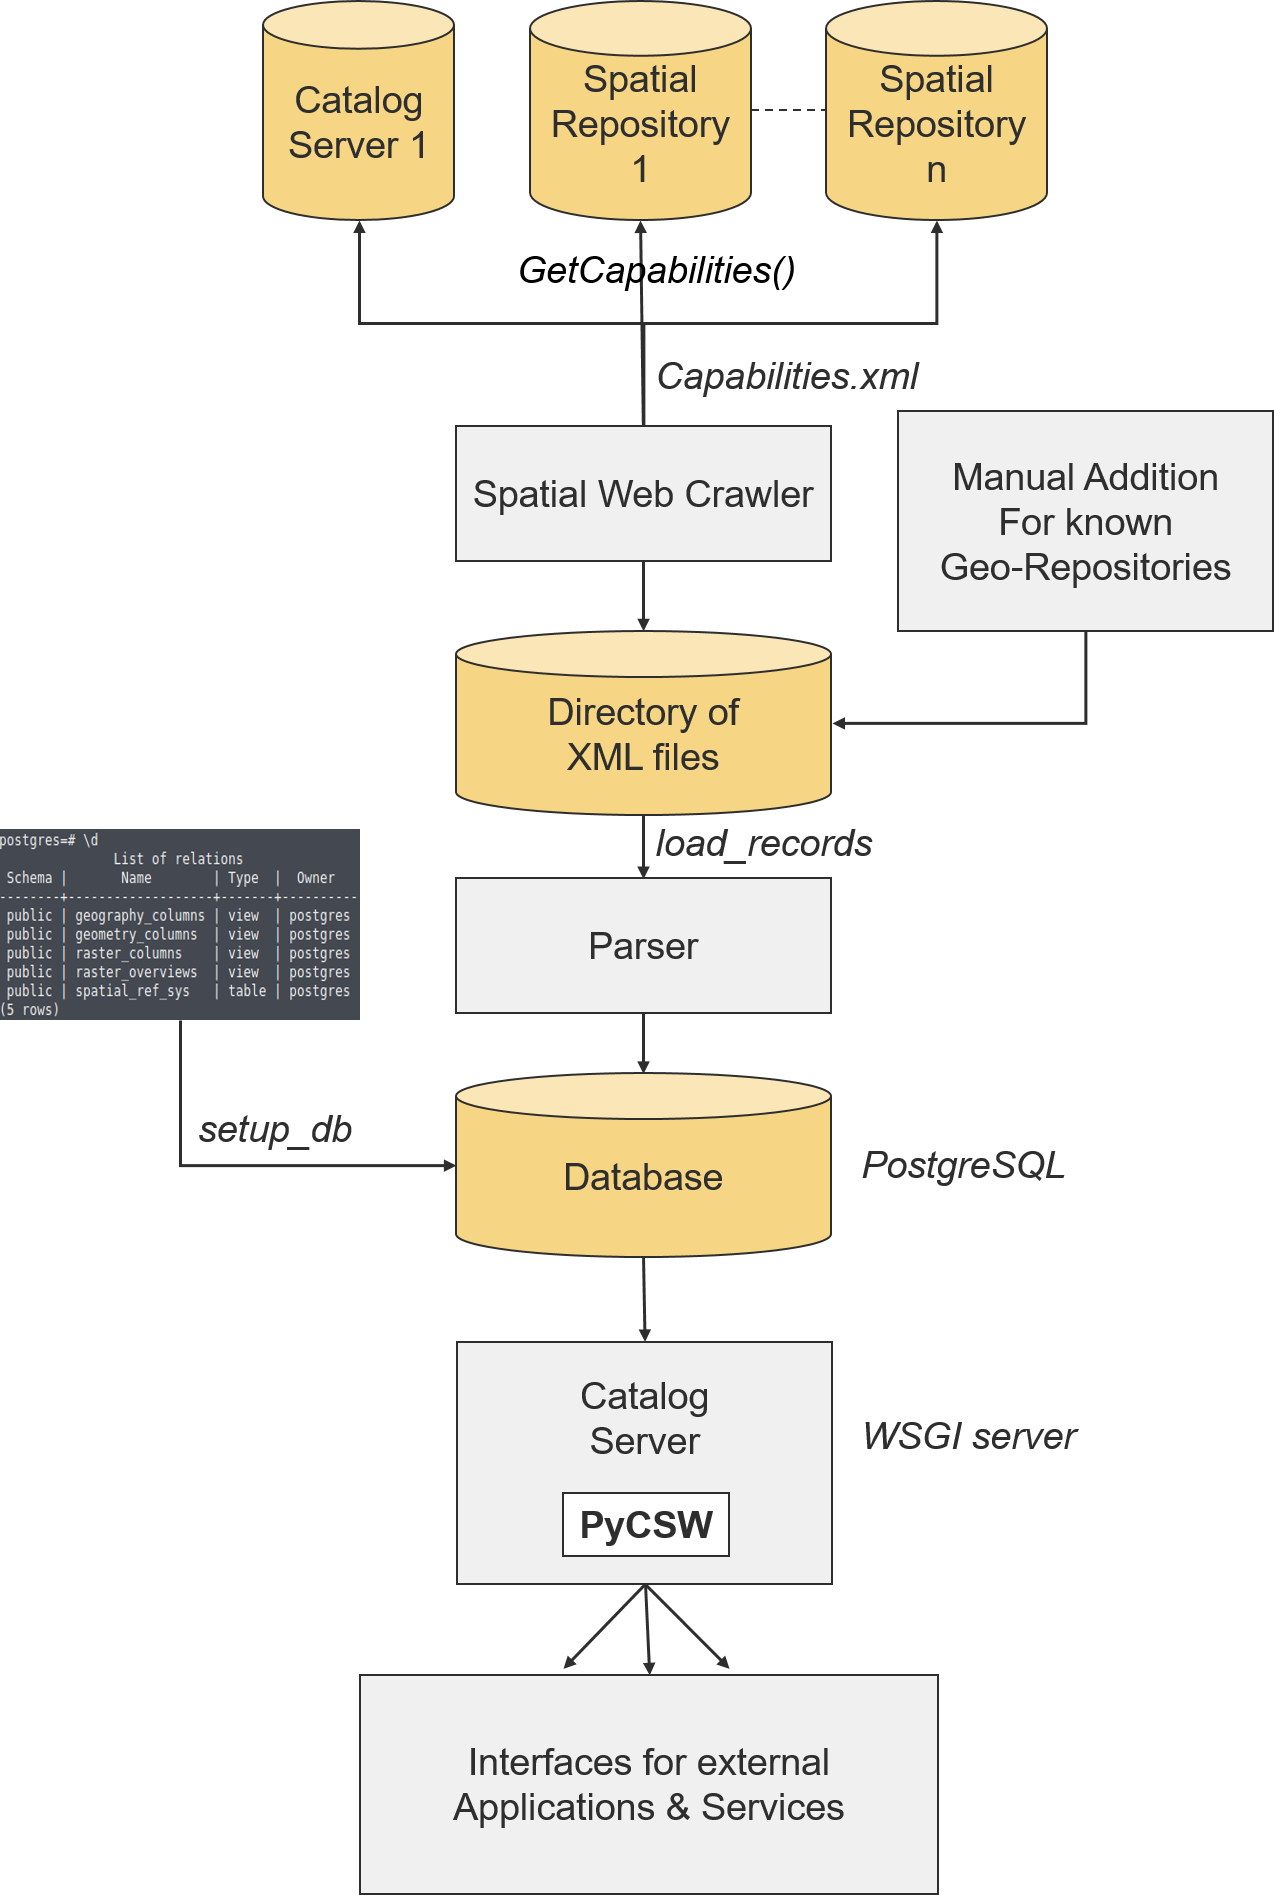
\includegraphics[width=\textwidth]{pix/Picture3}
 \caption{Architecture of Catalog Server}
 \end{figure}
 This information contains available operations, available layers and other useful information. This xml files are gathered in a folder containing xml files.\\



% \begin{figure}[h]
%   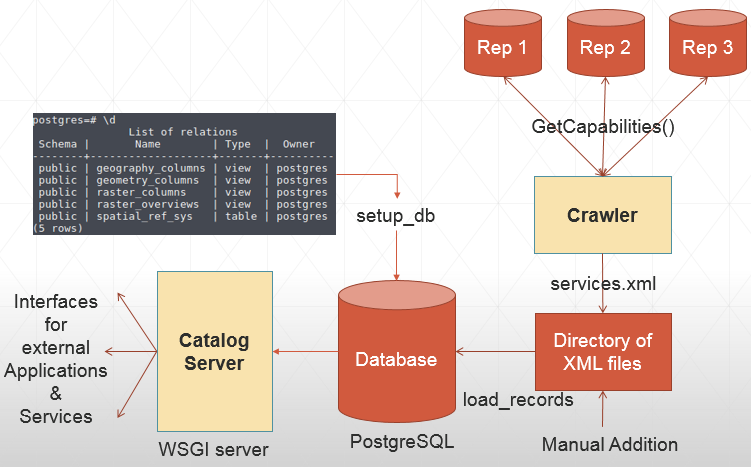
\includegraphics[width=\textwidth]{7}
%   \caption{Architecture of Catalog Service}
% \end{figure}

\par No of spatial repositories in the web is significantly lower than other type of services and servers. It can happen that it might take a significant amount of time to gather practically good number of geo-servers. For this reason, this files can be added by the spatial web crawler or it can be added manually.
\newline
\par This xml files are then loaded into the database for faster and efficient retrieval operation. For database we can use either of MySQL, PostgreSQL or SQLite. But MySQL and SQLite does not offer inherent data structures and operations support for spatial data. SQLite is also meant for light weight databases, whereas here the no of request-reply and data transfer can be very high. For these reasons it is better to choose PostgreSQL database system to store data for the catalog service. PostgreSQL offers high scalability and offers inherent support of spatial data types and operations.\newline
\par Catalog Service is hosted on \textit{Web server gateway interface (WSGI)} server. We can also use other deployment servers like Apache. Main reason for choice of server as WSGI is that, WSGI integrates well with python. It is build on python. It is useful for request-reply type ordinary web interfaces and it is efficient for file transferring on other protocols. A python program admin.py is hosted on WSGI server, which takes the metadata information from the database and replies in response to GetCapabilities() request. When working on a particular request for a repository like GetMap(), the catalog service acts as a mediator between client and the repository on which the data is hosted. It converts the request taken by WSGI server converts it into standard OGC compliant WMS or WFS call, and accesses data from original repository from where data is hosted.


\section{Implementation}
There are two types of implementation done to implement catalog service module. First implementation covers $PyCSW$ python catalog service for web and second implementation makes use of $GeoServer$ open source tool for sharing spatial data. Difference between two type of tools is while PyCSW offer great functionalities and most of the OGC compliant services, GeoServer also offers more data type support to load repository from and a management console for admin to maintain Geo-registry. We will take a look at both type of solutions here.

\subsection{Crawler Module}

In first stage implementation, we first crawl through open web using the spatial web crawler discussed in the above chapter. The crawler checks if the given server provides geospatial services or not. If the server is a geospatial repository then it collects all the metadata information about the repository and stores it in a form of a xml files. Standard OGC compliant service calls are used for collecting metadata information about found registry. Here in the figure we can see there are three repositories which have been crawled by the crawler. The information about these repositories are stored in a xml files called services.xml. The no of geoservers and registries are very less in the open web compared to other kind of services, for this reason it might take a long time to crawl and find significant amount of registry services for our catalog service. To handle this problem, manual addition option is used. We can manually add popular geoservers and registry services to the services.xml files. We know that geoservers reply in xml response when called for a $GetCapabilities$ request. We can use this property and manually add popular geo-registries beforehand to the set of xml files. So in the summary, the first stage crawls the web and stores corresponding set of services files into one place.
\newline
\par For this, python based crawler module program is used. It takes a set of seed URLs, checks if the URL can built object of OGC compliant WMS or WFS object. If it can build OGC WMS object then, crawler requests for capabilities file, and stores it in set of xml files.


\subsection{Database Setup}
In second step, These set of xml files are used to populate database. Here various type of databases can be used. I have tried databases like MySQL, SQLite and PostgreSQL. In our approach I have used PostgreSQL because it offers geospatial properties and services inherently. Other databases do not offer inbuilt services for spatial data. PostgreSQL database offers PostGIS extension, which are a set of libraries to extend PostgreSQL database into spatial database. For adding PostGIS to PostgreSQL, go to PostgreSQL shell psql and create a extension, PostGIS. 

\begin{center}
\textit{CREATE EXTENSION POSTGIS;}
\end{center}

\par Once this is done, import all of the services,xml files into the database. Create structured tables and schema for maintaining spatial data. For this purpose \textit{setup\_db} command is used from catalog service module.

\begin{figure}[h]
\centering
  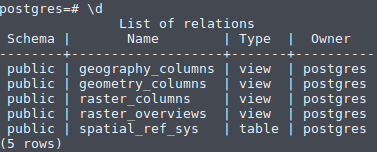
\includegraphics[width=0.8\textwidth]{8}
  \caption{List of relations}
\end{figure}

\par Here four tables are built to store and index spatial data efficiently. Those are, $geometry\_columns, records$ , $spatial\_ref\_sys$ and $spatial\_ref\_sys\_srid\_seq$. This tables are then used by the catalog server to publish and query available data. When a external entity queries catalog server for Get Capabilities request, the catalog server replies with the services file which contains all the information about all the geo-servers it has crawled till now. Thus it contains all the layer information and data crawled from the Internet. This makes it a single point of resource access. Data from xml files is parsed and stored into respective relations. For this \textit{load\_records} command is used from admin.py module within PyCSW. These tables are used to store parsed spatial features from the spatial repositories.

\subsection{Catalog Service}
Catalog service takes all available data from the database and creates a metadata capabilities file. It acts as a mediator between repositories which actually contains the data and the client. When a client requests for a query or a metadata service, catalog service checks if the database contains the information. If metadata information is requested, it replied directly to the client with the necessary files or response.\\
\begin{figure}[h]
\centering
  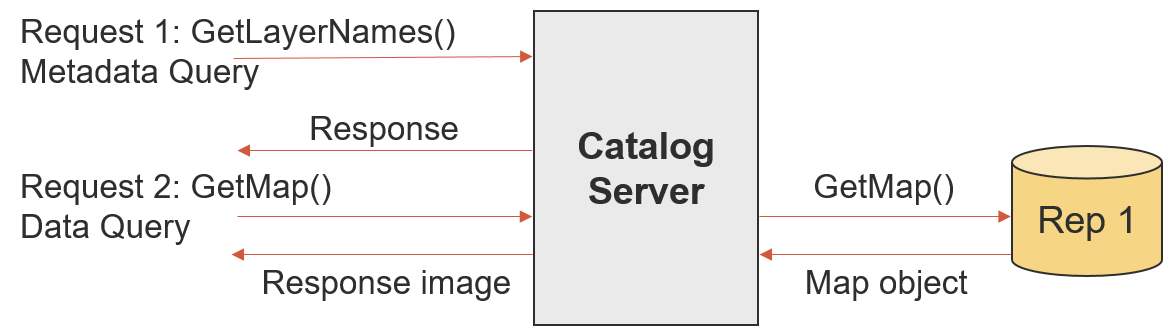
\includegraphics[width=\textwidth]{pix/Picture5}
  \caption{Catalog Service as a mediator}
\end{figure}
\par In case of query requiring actual data instead of the metadata, the catalog service resolves the source from which the data is available and brings the data back to the requester client. In this case, the catalog service acts as a mediator between client and the data source, acting just as a catalog. Here the catalog service is implemented via GeoServer. GeoServer takes the crawled layers from web map service and loads it into catalog.

\subsection{Query Processing}
When a query or request for the data is processed by the catalog service, it acts as a mediator between client and the repository from which the data is intended. It creates a object of the required service and requests for the object on behalf of the client. Client authorizes to the catalog service and catalog service authorizes itself to the data repositories for the transfer of data. Catalog service takes the object response from the repository and send it in response to client in client specified format. For metadata queries the catalog service retrieves data from database via object relational mappings in programming paradigms, this helps when having a multiple references to same object or feature. This method is used for retrieval of the features. How the featured are retrieved and presented are discussed further in the chapter 5.


%%%%%%%%%%%%%%%%%%%%%%%%%
\section{Extending catalog service with cloud characteristics}
A key logical step to scale catalog service for the larger audience is to make a cloud based implementation. Cloud based implementation has characteristics like scaling horizontally, high availability and dynamic dispatch of machines. To achieve the effects of scalability and high availability, we can make use of $load\_balancer$, $load\_balancer$ is a machine that acts as a middleware between client request and actual catalog servers. It forwards the request to one of the servers based on some qualitative features.
\newline
\begin{figure}[h]
    \centering
    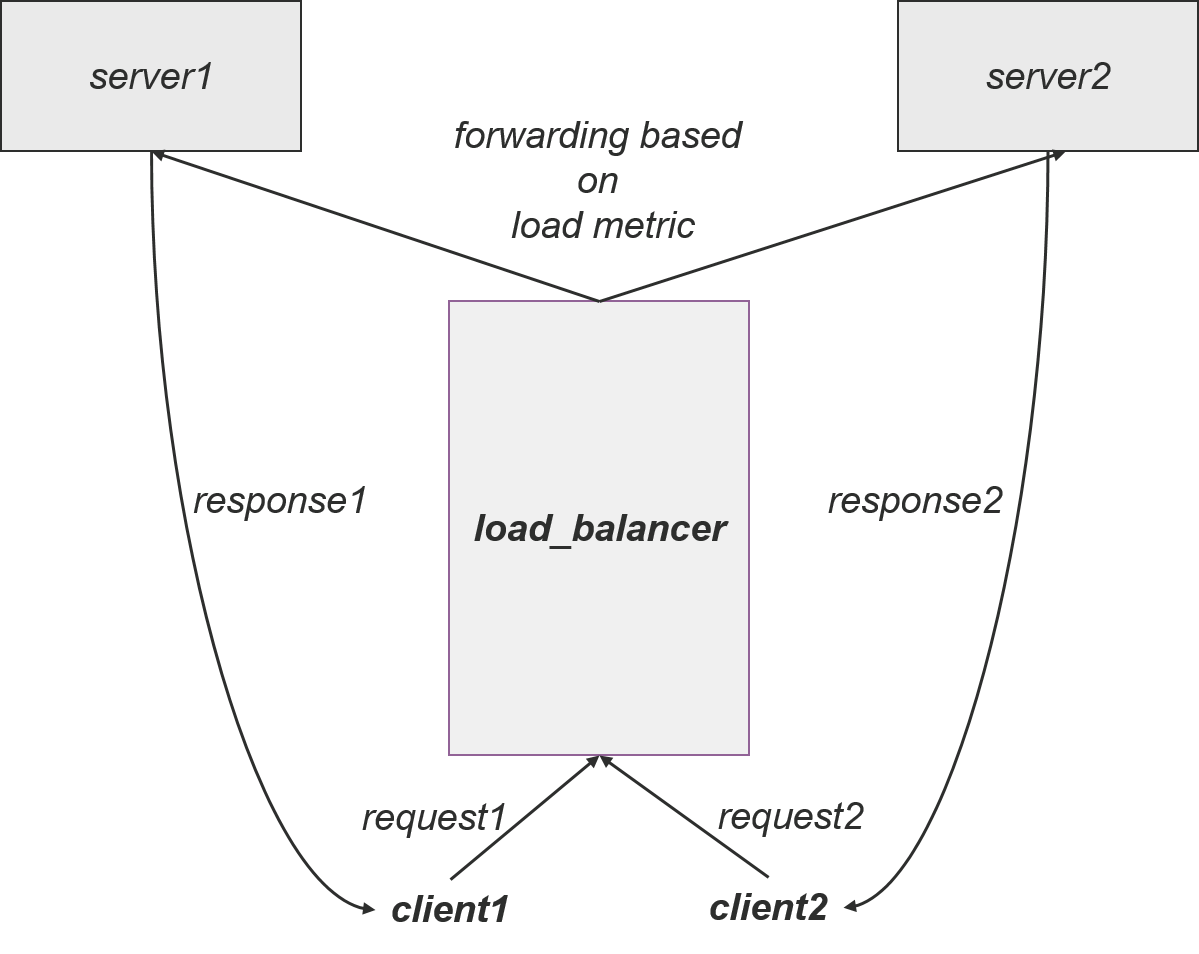
\includegraphics[width=0.7\textwidth]{pix/Picture7}
    \caption{load balancer implementation}
    \label{p7}
\end{figure}


\par In our approach, we have started by building a $load\_balancer$ which balances the requests between multiple available given geoservers. These geoservers are cloned to provide similar functionality but high availability. $load\_balancer$ detects which server has low number of requests compared to others and forwards the request to particular server. Actual servers are transparent to the end users. Interface between client and the geoservers is the $load\_balancer$. It acts as a gateway for connecting with the geoservers. In our test implementation, we have created two instances of geoservers and run similar repositories on each of them. The client connects to the $load\_balancer$ which acts as a gateway for the actual geoservers. It gets the reply back from the actual servers and sends it to requesting clients. $load\_balancer$ can also restrict or allow certain users grant on certain function and not all of them, thus here $load\_balancer$ also acts as a control panel and authorization entity for the access control.
\newline
\begin{figure}[h]
    \centering
    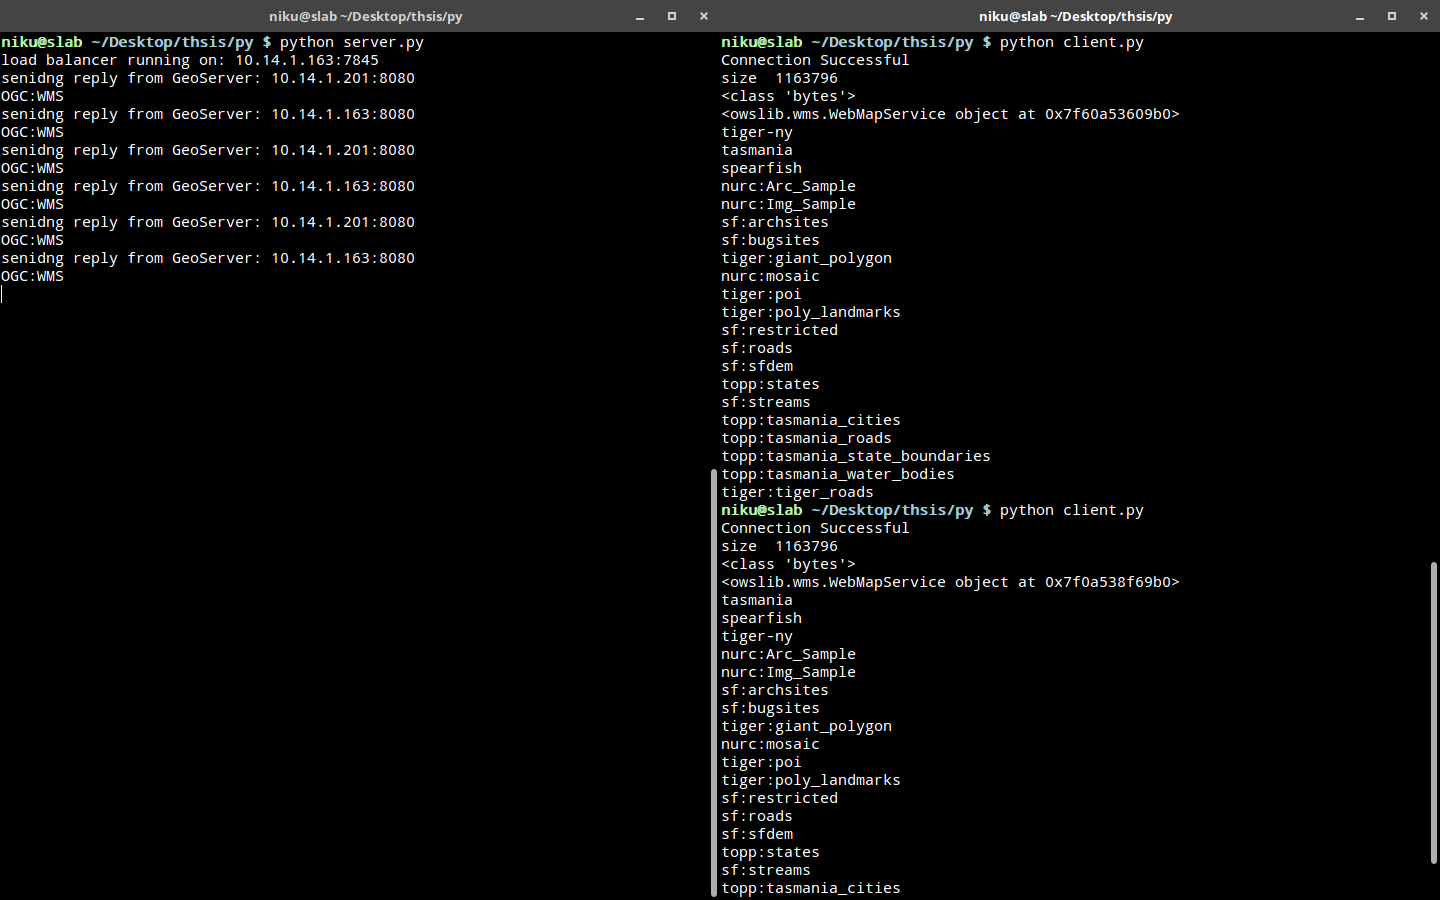
\includegraphics[width=\textwidth]{pix/p13}
    \caption{load balancer preliminary results}
    \label{p13}
\end{figure}
%%%%%%%%%%%%%%%%%%%%%%%%%
\section{Results}
Here are some results from the projects that explains and elaborates what kind of information can be get from catalog service. We have connected to GeoServer instance that is locally hosted. Note that many more richer services can be added to the platform to extend it's functionality.

\begin{figure}[h]
    \centering
    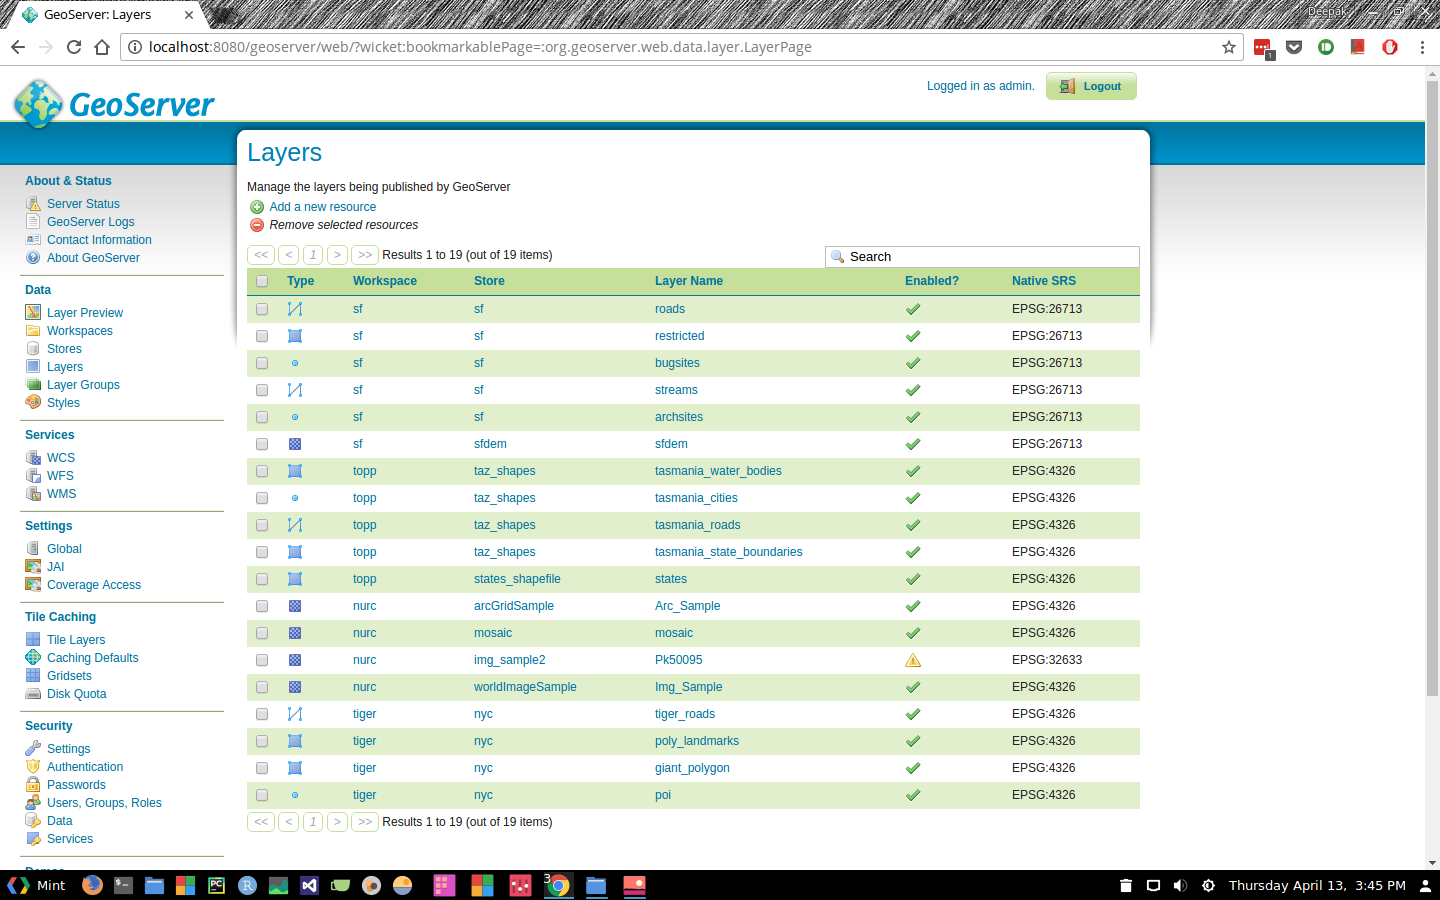
\includegraphics[width=\textwidth]{pix/p8}
    \caption{GeoServer Implementation}
\end{figure}

\begin{itemize}

\item Information about service metadata : OGC:WMS\\
This shows that registry is capable of providing OGC compliant web map service type of service to the user.\\

\item Title : GeoServer Web Map Service\\
Title gives information about title of the server hosting web map service.

\item List of available layers
\begin{enumerate}
\item kgp:POPULATION 
\item kgp:bnk\_block\_boundary 
\item kgp:bnk\_block\_hq 
\item kgp:bnk\_district\_boundary 
\item kgp:bnk\_drainage 
\item kgp:bnk\_grampanchayat\_boundary 
\item kgp:bnk\_mouza\_boundary 
\item kgp:bnk\_road
\item tasmania
\item spearfish
\item tiger\-ny
\item nurc:Arc\_Sample
\item nurc:Img\_Sample
\item sf:archsites
\item sf:bugsites
\item tiger:giant\_polygon
\item nurc:mosaic
\item tiger:poi
\item tiger:poly\_landmarks
\item sf:restricted
\item sf:roads
\item sf:sfdem
\item topp:states
\item sf:streams
\item topp:tasmania\_cities
\item topp:tasmania\_roads
\item topp:tasmania\_state\_boundaries
\item topp:tasmania\_water\_bodies
\item tiger:tiger\_roads
\end{enumerate}

This shows the list of available data in the form of layers. Each layer represents data of a geographic location from a view point. Multiple layers can be overlapped on each other to better understand the data. Each layer contains multiple features in itself. 

\item Available operations (WMS)
\begin{enumerate}
\item GetCapabilities 
\item GetMap 
\item GetFeatureInfo 
\item DescribeLayer 
\item GetLegendGraphic 
\item GetStyles 
\end{enumerate}

Gives details about the operations that can be performed by the geoserver. For example, DescribeLayer provides information about a particular layer. GetMap returns a map of layer in multiple available formats. 

\item GetMap\\
\begin{figure}[H]
	\centering
  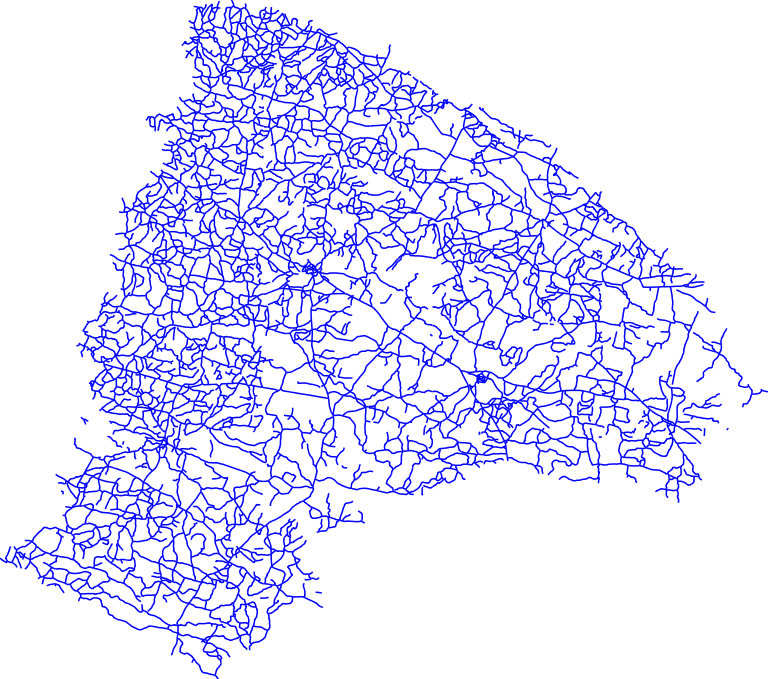
\includegraphics[width=0.7\textwidth]{bnk}
	\caption{Map of KGP BNK ROAD}
\end{figure}
Returns a map of particular layer. Can be superimposed to another map for better visualization. GetMap supports multiple options like name of layer(s), styles, transparency, bounding box, size and format like jpeg, png or pdf. 
\item DrawMap\\
DrawMap overlays different map images on top of each other to better visualize and analyze the effect of desired operation. For example, it can be used to find area affected by flood, or to find division of regions based on religion.\\
\begin{figure}[H]
	\centering
  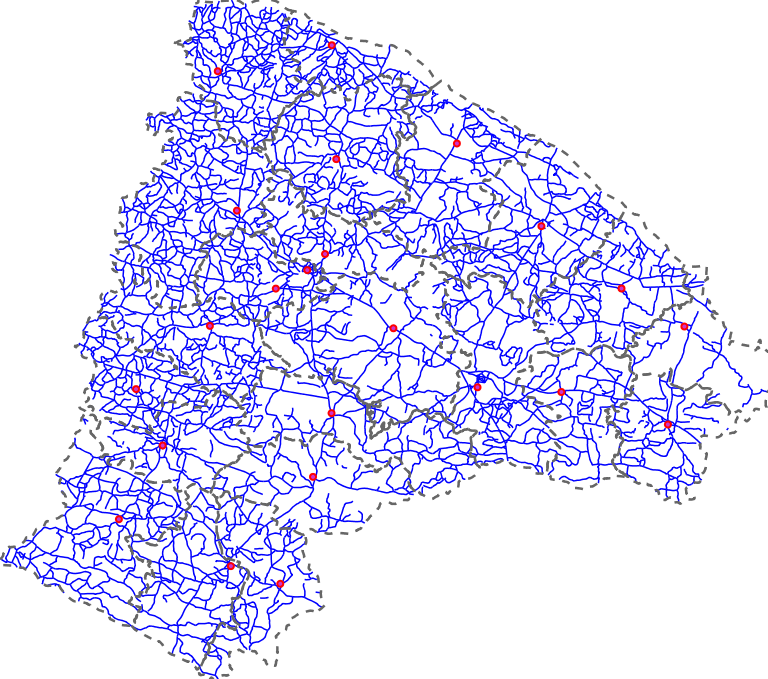
\includegraphics[width=0.7\textwidth]{9}
	\caption{Overlay of KGP BNK ROAD, Block HQ \& Boundary Layers}
\end{figure}
User can specify options to get the result image in desired format.\\
Options:\\
Layers = \{ kgp:bnk\_road, kgp:bnk\_block\_hq, kgp:bnk\_block\_boundary \}\\
Width = 768\\
Height = 679\\
Format = image/png

\item Information about specific layer: 
\begin{itemize}
\item Title --- POPULATION 
\item Name --- kgp:POPULATION 
\item Is Queryable --- 1 
\item Is Opaque --- 0 
\item Bounding Box ---  
\item minx --- 68.52669525146484 
\item miny --- 8.086045265197754 
\item maxx --- 97.3387680053711 
\item maxy --- 35.8697509765625
\end{itemize}
Provides information about a particular layer, for example, name of the layer, title, bounding box information etc.

\item Similar information can be found for web feature service, for example, supported operations in WFS.
\begin{enumerate}
\item GetCapabilities
\item DescribeFeatureType
\item GetFeature
\item GetGmlObject
\item LockFeature
\item GetFeatureWithLock
\item Transaction
\end{enumerate}

\end{itemize}

% \chapter{Introduction}
Wireless sensors are devices capable of sensing some physical data, capable of doing limited processing and communicate with other sensors or devices in its communication range. The set of wireless sensors deployed in a field for a common purpose forms a \textit{wireless sensor network (WSN)}. Wireless sensor networks are widely used in different application domains such as surveillance (military and civilian), environmental monitoring, chemical and toxic detection, habitat monitoring, healthcare monitoring,  industrial and commercial applications which includes home appliances. The very basic component of a WSN is the wireless sensor or wireless sensor node. It is so called wireless because the nodes are communicate with each other or its base station using any one of the wireless technologies. 

A typical wireless sensor node consists of the following subsystems such as a sensor to sense the physical quantity, an embedded processor or microcontroller, small amount of memory (typically few megabytes), a tranceiver for communication and a battery. A wireless sensor network is called as a network because each of the wireless sensors nodes are communicating to its neighbour sensor nodes and route the data to the base station in a multihop manner. There can be a \textit{sink node} in a group of sensor nodes which has got higher communication range to connect to the base station. In such cases sensor nodes communicate to the nearest sink node through its neighbours. WSN can be treated as a special case of adhoc networks.

There are several research problems in the field of wireless sensor networks. The main areas are communication and routing, coverage, localization, energy conservation, sleep scheduling and data aggregation. Even though energy conservation is listed as one of the research area in wireless sensor networks, it is considered as one of the design constraint for all other problems in WSN. Coverage is one of the important area in the field of wireless sensor networks. 

\textit{Mobile wireless sensor network} is a kind of wireless sensor network, where the sensor nodes are mobile. A sensor node which is capable of moving as well as sensing and communicating is known as mobile sensor node.There are networks with stationary nodes and mobile nodes together, commonly known as mixed wireless sensor networks\cite{lambrou2012testbed}.  
Due to the advancements in robotics, automation and battery technologies, sensor nodes are coming up with the capability of moving within the area of interest. Again the mobility is limited because of the high power consumption requirement for the movement. 
Mobility introduces a new set of challenges in all the research areas of wireless sensor networks. In case of coverage, the area covered by mobile node is known as dynamic coverage area  \cite{mahboubi2013distributed}. 

\textit{Area Coverage} is how well all the points in the area of interest are sensed by the nodes in the network. Some of the applications need not required to monitor the entire area continuously, instead periodic monitoring is sufficient. Periodic sensing of all points in the area of interest is known as \textit{area sweep coverage} \cite{gorain2013point}. Area sweep coverage in a mobile wireless sensor network with docking stations for recharging of mobile sensor nodes is the work in this thesis.



\section{Coverage in Wireless Sensor Networks}

Coverage is about how well the \textit{area of interest (AoI)} sensed by the sensor network. In wireless sensor network, coverage always refers to sensing coverage i.e., the field under the sensing range of the the sensor node. The communication range is different, that refers the maximum distance a sensor node can communicate with other nodes.
Coverage problems are classified into three categories based on the sensing need in the area of interest. They are area coverage, target coverage and barrier coverage. The type of coverage for a wireless sensor network is decided based on the application. \textit{Area Coverage} is how well all the points in the area of interest are sensed by the nodes in the network. Area coverage is also known as \textit{blanket coverage}. If the sensing requirements of a WSN is for sensing some specific points or targets in the area of interests, then the coverage is \textit{target coverage}. It is also known as \textit{point coverage}.  The third category is barrier coverage. In barrier coverage applications, the sensor nodes have to sense only the barrier strips of the AoI. The deployment of the sensors are controlled over the boundary region. 

The design phase, deployment phase and maintenance phase of the WSNs differ for each class of coverage. During the design phase, the optimal positioning of the sensor nodes to enhance the coverage is considered. Algorithms are designed for positioning of the sensor nodes based on the area of interest and the sensing range of the sensor nodes. There are basically two types of deployments. They are deterministic and random deployment. The sensor nodes are placed in the predetermined positions in deterministic deployment, but in case of random deployment, sensors are distributed in the area by deploying from aeroplane or similar methods. Then sensor nodes form the network and different algorithms are used for sleep scheduling and movement of sensor nodes to enhance coverage. The purpose of coverage algorithms in the maintenance phase is to find the coverage holes in the network and find solution to enhance the coverage either by deploying more sensor nodes or moving the sensor nodes to cover the holes \cite{vecchio2015improving}. 

It is difficult to cover the entire area in some of the applications because achieving the node density for a deployment is not possible always. Then certain percentage of the area or points or the barrier region will be covered based on the probability of events to occur in the region. This type of coverage is known as \textit{partial coverage} or \textit{p-percent coverage} \cite{mostafaei2015connected}. Another important coverage method is sweep coverage. The points or the areas are sensed by the sensor nodes in periodically. The interval of each sensing is decided based on the requirement of the application. The advantage of sweep coverage is minimum number of sensor nodes and reduced energy consumption. This is realized using either the help of mobile sensor nodes or by sleep scheduling of already deployed sensor nodes. More details of the approaches and algorithms in sweep coverage are discussed in literature survey section.

\section{Motivation}
The advancement in aerial robotics led to more innovations in the area of unmanned aerial vehicles like drones. These type of innovations can be made use in wireless sensor networks also. The mobility of mobile sensor nodes can be enhanced using these technologies. At the same time, the custom built drones can be used as a sensor node in a mobile wireless sensor network. Both of these approaches call for a mobile wireless sensor network with a sensor node with more flying capacity. But the higher energy consumption requirement also come along with these sensor nodes. So the concept of docking stations (recharging stations or refuelling stations) is introduced. These docking stations are present in the area of interest and mobile sensor nodes has to come to these stations and recharge during their movement for sensing the region.

The concept of docking stations in the area of interest, the charge scheduling of the mobile sensor nodes and trajectory design of each mobile sensor node lead to a whole new set of problems. Trajectory is the instantaneous position of the mobile sensor node with respect to time. Very little study is done in area sweep coverage as well as docking stations for recharging inside the area of interest. So both the problem of area sweep coverage and trajectory design based on the position of the docking stations is challenging. There are many applications like city surveillance, military surveillance and environmental monitoring can make use of the high capacity mobile sensor nodes and thus the quality of service can be improved to a great extend.
 
\section{Contribution}
Our aim is to design an optimal solution for area sweep coverage in mobile wireless sensor network where the docking stations are present inside the area of interest for the mobile sensor nodes to recharge or refuel during their movement to the area. The objective is to find the minimal cumulative distance travelled by all the mobile sensor nodes so as to cover the entire are of interest in each sweep interval. The intrinsic features of the problem and its complexities are analysed.

\section{Organisation of Thesis}
The thesis is organised as follows. Chapter 2 is literature survey. The detailed discussion about the works done in coverage in wireless sensor network is included. More elaboration is given for the studies and works in area coverage and sweep coverage of mobile sensor networks. Chapter 3 is problem definition. The problem statement and problem definition in mathematical form is given. This chapter also discuss the complexity and hardness of the problem.


%To start the new chapter in another page 
\newpage
\thispagestyle{empty}
%\cleardoublepage
 
%\chapter{Literature Survey}

The introduction of the coverage problems in wireless sensor networks is briefly discussed in the previous chapter. This chapter goes to the details of the wide range of works already done in this area and its advantage, improvements done by other researchers are discussed. The three main classes of coverage in WSN such as area coverage, point coverage and barrier coverage are discussed in detail. Various works done in the field of sweep coverage in wireless sensor networks particularly in point coverage is discussed. The definitions and studies in area sweep coverage in mobile wireless sensor networks is discussed in the last section.

Bang Wang \cite{wang2011coverage} defined the sensor coverage as follows. Sensor coverage models are abstraction models trying to quantify how well sensors can sense physical phenomena at some location, or in other words, how well sensors can cover such locations. Network sensing coverage, on the other hand, can be considered as a collective measure of the quality of service provided by sensor nodes at different geographical locations.

\section{Area Coverage}

\subsection{Area Coverage in MWSN}

\section{Target Coverage}

\section{Barrier Coverage}

\section{Sweep Coverage}

\subsection{Area Sweep Coverage}



%Sweep Period \cite{yang2013sweep}
%Sweep coverage either by sleep scheduling or by mobility.\\
%Point Sweep Coverage \cite{wang2011coverage} Discussion\cite{gorain2015approximation}
%all\cite{yang2013sweep}
%
%
%Difference between deployment point and docking station.\\ 
%Extensive discussion about all the works in this area.




% \chapter{Literature Survey}

The introduction of the coverage problems in wireless sensor networks is briefly discussed in the previous chapter. This chapter goes to the details of the wide range of works already done in this area and its advantage, improvements done by other researchers are discussed. The three main classes of coverage in WSN such as area coverage, point coverage and barrier coverage are discussed in detail. Various works done in the field of sweep coverage in wireless sensor networks particularly in point coverage is discussed. The definitions and studies in area sweep coverage in mobile wireless sensor networks is discussed in the last section.

Bang Wang \cite{wang2011coverage} defined the sensor coverage as follows. Sensor coverage models are abstraction models trying to quantify how well sensors can sense physical phenomena at some location, or in other words, how well sensors can cover such locations. Network sensing coverage, on the other hand, can be considered as a collective measure of the quality of service provided by sensor nodes at different geographical locations.

\section{Area Coverage}

\subsection{Area Coverage in MWSN}

\section{Target Coverage}

\section{Barrier Coverage}

\section{Sweep Coverage}

\subsection{Area Sweep Coverage}



%Sweep Period \cite{yang2013sweep}
%Sweep coverage either by sleep scheduling or by mobility.\\
%Point Sweep Coverage \cite{wang2011coverage} Discussion\cite{gorain2015approximation}
%all\cite{yang2013sweep}
%
%
%Difference between deployment point and docking station.\\ 
%Extensive discussion about all the works in this area.




% \chapter{Problem Formulation and Complexity Analysis}
\section{Problem Statement}
Consider an area of interest as a rectangular area, $\mathbb{A}$ and a set of static sensor nodes, $S=\{ s_1,...,s_p \}$ are placed in some locations in $\mathbb{A}$. Let $M=\{ m_1,...,m_q \}$ denote the set of \textit{mobile sensor nodes (MSNs)} and each mobile sensor node is attached to one of the \textit{docking  stations}. Let $D=\{ d_1,...,d_r \}$ is the set of docking stations that are located inside $\mathbb{A}$ and capable of providing charging facility for one or more mobile sensor nodes. Mobile sensor nodes move with a constant \textit{speed} and senses the field under their \textit{sensing range} throughout the move. Mobile nodes come back to the same docking station from where it started the sweep move. \textit{Sensing field} of a mobile sensor node or a static sensor node is considered as a circular disk with current location of the sensor node as the center of  the disk. The sensing range is the radius of the disk.

\textit{Minimum Distance Area Sweep Coverage Problem} is to find the \textit{trajectory} for mobile sensor nodes so as to cover $\mathbb{A}$ atleast once in a given time period by any of the sensor nodes  with minimal cumulative distance travelled by all the mobile sensor nodes. This time period is known as \textit{sweep interval} or  \textit{sweep period}. The instantaneous position of the mobile sensor node with respect to time is known as trajectory. The mobile nodes have to sweep cover the area that is not covered by the static sensors. Each mobile node has to dock at its designated docking station to charge up after the sweep.

\subsection{Minimum Distance Area Sweep Coverage Problem}

Let $T$ be the sweep period and $V$ be the constant speed of the mobile sensor nodes. Consider the area of interest is divided into grid of square cells of side length less than sensing range of the mobile sensor node. Suppose $N_r$ be the number of rows and $N_c$ be the number of columns, then there are total $N_r \times N_c$ cells in $\mathbb{A}$. Let $C$ be the set of cells in the grid, $C=\{c_1,...,c_n\}$.  The cells are numbered from left to right and then from top to bottom. Topmost left cell is numbered as $c_1$ and bottommost right cell is numbered as $c_n$. Each cell $c_i$ is represented as $\left( x_{c_i},y_{c_i} \right)$ where $x_{c_i}$ is the row number and $y_{c_i}$ is the column number of the cell $c_i$.
Each static sensor node $s_i$ will have a tuple associated with it as $\left\langle s_i, L_i^s, R_i^s \right\rangle$, where $L_i^s$ is the location of the static sensor node and is represented as a cell in $\mathbb{A}$, $R_i^s$ is the sensing range of the static sensor node $s_i$.
Each docking station $d_j$ will have a tuple associated with it as $\left\langle d_j,L_j^d, \beta_j, cap_j \right\rangle $, where $L_j^d$ is the location of the docking station and is represented as a cell in $\mathbb{A}$, $\beta_j$ is the charging rate per unit time, $cap_j$ is the charging capacity of the docking station i.e.,\ number of mobile sensor nodes that can be simultaneously charged.
Each mobile sensor node $m_i$ will have a tuple associated with it as $\left\langle m_i, R_i^m, \gamma_i, \delta_i, d_j \right\rangle$, where $R_i^m$ is the sensing range of $m_i$, $\gamma_i$ is the discharge rate of $m_i$ per unit distance, $\delta_i$ is the distance travelled by $m_i$ in terms of number of cells during a sweep and $d_j$ is the docking station where $m_i$ is attached.

The sweep period, $T$ is divided into $T$ time slots where [0-1] denotes the 1st time slot, [1-2] denotes the 2nd time slot,...,[T-1,T] denotes the $Tth$ time slot.
Assume that initially all the mobile sensor nodes are fully charged. Let $M_c$ be the \textit{maximum charge capacity} of each mobile sensor node. Total energy consumed by mobile sensor node $m_i$ in a sweep is $E_i = \delta_i \times \gamma_i$. Sensing and communication energy requirements are not considered for simplicity. The time required for the mobile sensor node $m_i$ to recharge from a docking station $d_j$ is $\lambda_{m_i,d_j} = E_i / \beta_j$. Let time taken by a mobile sensor node $m_i$ to finish its flight for a sweep be $\tau_m = \delta_i / \ V$.

\textit{Cell occupancy status} indicates the trajectory of the mobile sensor nodes and it can be represented as a set of variables $ \{ \phi_{t,c,m_i} \}$, where $ \phi_{t,c,m_i} = 1 $ indicates at time $t$ the mobile sensor node $m_i$ is located at cell $c$; otherwise $ \phi_{t,c,m_i} = 0 $.
\[
\phi_{t,c,m_i}=
%A
\begin{dcases}
1 & \text{if}\  \exists {m_i \in {M}}\ \ s.t. \ position(m_i, t) = c  \\
0 & \text{otherwise.}
\end{dcases}
\]


The objective is to design the trajectory and the recharge schedule for the mobile sensor node so as to  minimize the cumulative distance travelled $(\Delta)$ by mobile sensor nodes.

The output is the trajectory i.e., cell occupancy status as a set of variables $ \{ \phi_{t,c,m_i} \}$   and the charging schedule as a set of variables $\left\lbrace \chi_{m_i,d_j,t} \right\rbrace $ where $\chi_{m_i,d_j,t} = 1 $ indicates that mobile sensor node $m_i$ is charging at docking station $d_j$ at time slot $t$; otherwise $\chi_{m_i,d_j,t} = 0 $. The problem is formally specified as follows:\\

minimize\ \ \ 
$
\Delta = \sum\limits_{t \in T} \sum\limits_{c \in C} \sum\limits_{m_i \in M} \phi_{t,c,m_i}
$\\\\
subject to the following conditions
\begin{eqnarray}
\sum\limits_{t \in T} \sum\limits_{c \in C} \sum\limits_{m_i \in M} \phi_{t,c,m_i} \geq N_c 
\end{eqnarray}
\begin{eqnarray}
\forall{c\in C}\ \sum\limits_{t \in T} \sum\limits_{m_i \in M} \phi_{t,c,m_i} \geq 1
\end{eqnarray}
\begin{eqnarray}
\forall{t\in T}\ \forall{m_i \in M}\  \sum\limits_{c \in C} \phi_{t,c,m_i} \leq 1
\end{eqnarray}
\begin{eqnarray}
\forall{m_i \in M}\ \sum\limits_{t \in T} \sum\limits_{c \in C} \phi_{t,c,m_i} \times \gamma_i \leq M_c
\end{eqnarray}
\begin{eqnarray}
\forall{d_j \in D}\ \forall{t \in T} \sum\limits_{m_i \in M}{ \chi_{m_i,d_j,t} } \leq cap_j 
\end{eqnarray}\\
Constraint 1 specifies that the total cells to be covered in each sweep. Constraint 2 tells that the entire area should be covered i.e, every cells has to be visited once. Constraint 3 tells that same mobile sensor node should not be in two different cells at the same time. Constraint 4 indicates that maximum distance a mobile sensor node can travel after a full charging is limited to the maximum charge capacity, $M_c$ of the mobile sensor node. Constraint 5 specifies that at any time slot, the number of mobile sensor nodes scheduled for charging at a docking station should not be more than the capacity of the docking station. 

The movement of an MSN from one cell to another is restricted by the neighbour cell movement policy. Let $position \left( m_i, t \right)  = \left( x_{c_i} , y_{c_i} \right) $, then \\ $position \left( m_i, t+1 \right) =\left( x_{c_i}' , y_{c_i}' \right) $ where $ x_{c_i}-1 \leq x_{c_i}' \leq x_{c_i}+1$ and $ y_{c_i}-1 \leq y_{c_i}' \leq y_{c_i}+1$ for $ 1 \leq x_{c_i}' \leq N_r$  and $ 1 \leq y_{c_i}' \leq N_c$.

We refer this problem as Minimum Distance Area Sweep Coverage Problem (MinDistAreaSCov).

\subsection{NP-Completeness of MinDistAreaSCov Problem}
In this section, we define a restricted version of MinDistAreaSCov Problem where the static sensor nodes are not considered in $\mathbb{A}$. Also relax the number of docking stations i.e., there can be individual docking stations for each mobile sensor node. The number of docking stations and mobile sensor nodes can be same. We refer this restricted version of MinDistAreaSCov problem as \textit{R-MinDistAreaSCov Problem}. The output of R-MinDistAreaSCov is a set of variables  $ \{ \phi_{t,c,m_i} \}$, where $ \phi_{t,c,m_i} = 1 $ indicates at time $t$ the mobile sensor node $m_i$ is located at cell $c$; otherwise $ \phi_{t,c,m_i} = 0 $.

The R-MinDistAreaSCov problem is defined as follows:\\

minimize\ \ \ 
$
\Delta^{'} = \sum\limits_{t \in T} \sum\limits_{c \in C} \sum\limits_{m_i \in M} \phi_{t,c,m_i}
$\\

subject to the condition $\forall c \in C \sum_{t \in T} \sum_{m_i \in M} \phi_{t,c,m_i} \geq 1 $. The decision version of R-MinDistAreaSCov problem (D-R-MinDistAreaSCov) is to decide that given the number of mobile sensor nodes $q$, whether there exist an assignment of 0 or 1 to the set of variables $\phi_{t,c,m_i}$ such that $\forall c \in C \sum_{t \in T} \sum_{m_i \in M} \phi_{t,c,m_i} \geq 1 $.  Then we show that \textit{D-R-MinDistAreaSCov} problem is NP-Complete by reducing it from \textit{decision version of set cover problem (D-SCP)} which is a known NP-Complete problem. This implies that MinDistAreaSCov problem is also NP-Complete. \\\\
The decision version of set cover problem (D-SCP) is defined as follows:\\

\textbf{D-SCP:}
Let $U=\{ 1,2,...,n \}$ be the universal set  and a set $X=\{1,2...,m\}$. Let $S_i$ be a subset of  $U$ such that $S_i \subseteq U$ and $\bigcup_{i \in X} S_i=U$. Is there an $H$ for a given $k$ where $k$ is a positive integer such that $H \subseteq X$, $\bigcup_{i \in H} S_i=U$ and $ \mid H \mid = k ? $ 
 \\\\
\textbf{\textit{Theorem 1.}} \textit{The D-R-MinDistAreaSCov problem is NP-Complete}.\\\\
\textbf{\textit{Proof.}} First of all let us prove D-R-MinDistAreaSCov $\in$ NP. Given a certificate of the problem, we can find whether all the cells are covered by atleast one mobile sensor node by finding the sum of $\phi_{t,c,m_i} $ for each cell over the time period T. The result is cell occupancy count for each cell. If this individual sum for each and every  cell is greater than or equal to one then the entire area is covered using $q$ mobile sensor nodes. Thus, the certificate can be verified in polynomial time.

Now we prove that D-R-MinDistAreaSCov is NP-hard by showing that D-SCP $\leq_p$ D-R-MinDistAreaSCov. The reduction algorithm takes an instance of D-SCP, and produces an instance of D-R-MinDistAreaSCov in polynomial time as follows:

Let $A$ be an input instance of D-SCP with $U=\{1,2,...,n\}$ as universal set, $X=\{1,2,...,m\}$ i.e., $m$ number of subsets $S_i \subseteq U$ and a positive integer $k$. Then the instance $B$ of D-R-MinDistAreaSCov is defined by setting (1) $C=\{1,2,...,c_n\}$ as set of all cells in the grid, (2)Consider $C_{m_i}$ as the set of cells occupied in a sweep by an MSN as the subset of $C$. (3)There can be $m$ number of MSNs and (4)cover entire area (cells) with $q$ number of MSN i,e., $q=k$. 

We first show that a solution of  D-SCP  gives  a  solution  of  D-R-MinDistAr- eaSCov. Let $H'$ be a solution of D-SCP i.e., $H' \subseteq X$ gives the subsets for covering $U$ and $\mid H' \mid = k$. By our reduction elements of $H'$ are $C'_{m_i}$ i.e., cells covered by each $m_i$ are subsets of $C$. $C'_{m_i}$ is computed from the output instance $\phi{'}_{t,c,m_i}$ for every MSN of D-R-MinDistAreaSCov. $q = k$ is the number of mobile sensor nodes. If set cover is possible with $k$ subsets of $S_i$, then entire area (cells) can be covered with $q$ MSNs. Therefore $\bigcup_{i=1}^{q} C'_{m_i} = C$. Hence, $C'_{m_i}$ is a valid solution of D-R-MinDistAreaSCov. Hence, a solution of D-SCP gives a solution of D-R-MinDistAreaSCov.

We next show that the solution of D-R-MinDistAreaSCov gives a solution of D-SCP.  Solution of D-R-MinDistAreaSCov gives the cell covered by each MSN $m_i$ at time $t$ as $\phi{'}_{t,c,m_i}$. $C'_{m_i}$ where $1 \leq i \leq q$ gives the set of cells covered by each MSN $m_i$. This is deduced from $\phi{'}_{t,c,m_i}$. Avoid the notion of time slot and treat the cells covered during entire sweep as the elements of set $C'{m_i}$.  $\bigcup_{i=1}^{q} C'_{m_i} = C$ i.e.,entire area of interest is covered.

From this, we will construct $H'$ as follows. Consider $C$, set of all cells in the area of interest as $U$ in D-SCP and $C'{m_i}$ as $S_i$ where $i$ in  $H'$, the set of subsets which cover $U$. $\mid H' \mid$ is $q$, the number of MSNs and $\{S_i\}$ is equivalent to $\{C'_{m_i} \}$. Hence,  $\mid H' \mid = k$ is a valid solution of D-SCP. Hence, a solution of D-R-MinDistAreaSCov gives a solution of D-SCP.

Hence, we have shown that for the reduction proposed, a valid solution of D-SCP gives a valid solution of 
D-R-MinDistAreaSCov and a valid solution of D-R-MinDistAreaSCov gives a valid solution of D-SCP. Hence, D-R-MinDistAreaSCov is NP-Complete.




% \input{formu}
% \input{result}
% \include{concl}
% \cleardoublepage

% A file for citations not appearing in the document itself.
% \input{nocites}
% 
% \singlespacing

%\bibliographystyle{unsrt}

% \bibliographystyle{plain}
% \bibliography{wsn}

% \begin{thebibliography}{5}
\begin{thebibliography}{5}
%%%%%%%%%%% 1
\bibitem{l1}
Sonal Patil, Shrutilipi Bhattacharjee, and Soumya K. Ghosh. \textquotedblleft A spatial web crawler for discovering geo-servers and semantic referencing with spatial features\textquotedblright.\ In \textit{International Conference on Distributed Computing and Internet Technology}, pp. 68-78. Springer International Publishing, 2014.

%%%%%%%%% 
\bibitem{l2}
Li, Wenwen, Chaowei Yang, and Chongjun Yang. \textquotedblleft An active crawler for discovering geospatial web services and their distribution pattern - A case study of OGC Web Map Service\textquotedblright.\ \textit{International Journal of Geographical Information Science} 24, no. 8 (2010): 1127-1147.

%%%%%%%%%%%
\bibitem{l3}
Najork, Marc.\textquotedblleft Web crawler architecture\textquotedblright.\ In \textit{Encyclopedia of Database Systems}, pp. 3462-3465. Springer US, 2009.

%%%%%%%%%%% may not be useful
\bibitem{l4}
Ahlers, Dirk, and Susanne Boll.\textquotedblleft Location-based Web search\textquotedblright.\ In \textit{The Geospatial Web}, pp. 55-66. Springer London, 2009.

%%%%%%%%%%%
\bibitem{l5}
Li, W., C. Yang, D. Nebert, R. Raskin, P. Houser, H. Wu, and Z. Li.\textquotedblleft Semantic-based web service discovery and chaining for building an Arctic spatial data infrastructure\textquotedblright.\ \textit{Computers \& Geosciences} 37, no. 11 (2011): 1752-1762.

%%%%%%%%%%%
\bibitem{l6}
Jiang, Jun, Chong-jun Yang, and Ying-chao Ren.\textquotedblleft A spatial information crawler for opengis wfs\textquotedblright.\ In \textit{Sixth International Conference on Advanced Optical Materials and Devices}, pp. 71432C-71432C. International Society for Optics and Photonics, 2008.

%%%%%%%%%%%
\bibitem{l7}
\textit{http://geopython.github.io/pycsw-workshop/}

\bibitem{l8}
\textit{https://geopython.github.io/OWSLib/}

%%%%%%%%%%%
\bibitem{l9}
Lopez-Pellicer, Francisco J., et al.
\textquotedblleft Discovering geographic web services in search engines\textquotedblright.\
\textit{Online Information Review} 35.6 (2011): 909-927.

\bibitem{l10}
\textit{https://github.com/geoserver/geoserver}

\bibitem{l11}Yiu, Man Lung, Hua Lu, Nikos Mamoulis, and Michail Vaitis.\textquotedblleft Ranking spatial data by quality preferences\textquotedblright.\ \textit{IEEE Transactions on Knowledge and Data Engineering} 23, no. 3 (2011): 433-446.

\bibitem{l12}
Hjaltason, Gisli, and Hanan Samet.\textquotedblleft Ranking in spatial databases\textquotedblright.\ In \textit{Advances in Spatial Databases}, pp. 83-95. Springer Berlin/Heidelberg, 1995.

\bibitem{l13}
\textit{https://github.com/karimbahgat/Pyqtree}

\bibitem{l14}
Paul, Manoj, and S. K. Ghosh.\textquotedblleft An approach for service oriented discovery and retrieval of spatial data\textquotedblright.\ In \textit{Proceedings of the 2006 international workshop on Service-oriented software engineering}, pp. 88-94. ACM, 2006.

\bibitem{l15}
Nogueras-Iso, Javier, Francisco Javier Zarazaga-Soria, Ruben Bejar, P. J. Alvarez, and Pedro R. Muro-Medrano.\textquotedblleft OGC Catalog Services: a key element for the development of Spatial Data Infrastructures\textquotedblright.\ \textit{Computers \& Geosciences} 31, no. 2 (2005): 199-209.

\bibitem{l16}
Jones, Christopher B., Alia I. Abdelmoty, David Finch, Gaihua Fu, and Subodh Vaid.\textquotedblleft The SPIRIT spatial search engine: Architecture, ontologies and spatial indexing\textquotedblright.\ In \textit{International Conference on Geographic Information Science}, pp. 125-139. Springer Berlin Heidelberg, 2004.

\bibitem{l17}
Lopez-Pellicer, Francisco J., Aneta J. Florczyk, Ruben Bejar, Pedro R. Muro-Medrano, and F. Javier Zarazaga-Soria.\textquotedblleft Discovering geographic web services in search engines\textquotedblright.\ \textit{Online Information Review} 35, no. 6 (2011): 909-927.

\end{thebibliography}

%%%%%%%%%%%
% \bibitem{latexcompanion8}
% Suakanto, Sinung, et al.
% \textit{Building crawler engine on cloud computing infrastructure.}
% Cloud computing and social networking (ICCCSN), 2012 international conference on. IEEE, 2012.
% \end{thebibliography}


% If you have no appendices, remove the following two lines.
% If you have more appdences, add them as necessary.
% \appendix
% \include{apdxa}

\end{document}
